\chapter{Simulating SMELLIE Events}\label{chap:beam_profiling}
\setlength{\epigraphwidth}{.6\textwidth}
\epigraph{Max Power : \textit{Kids. From now on there are three ways of doing things: the right way, the wrong way, and the Max Power way.}\\
Bart Simpson : \textit{Isn't that just the wrong way?}\\
Max Power : \textit{Yes, but faster!}}{\textsc{The Simpsons}}
\setlength{\epigraphwidth}{.4\textwidth}
Critical to extraction of scattering information from SMELLIE data is an accurate MC simulation of the SMELLIE system. By modelling the laser light emission into the detector correctly, we can simulate how SMELLIE light will be impacted by changing scattering lengths in the detector. Because of the complexity of the optics of the optical fibres used to direct the laser light into the detector, a given SMELLIE event is simulated as a partially-collimated ``flash'' of visible photons emanating from the emission point of the fibre into the detector. This flash then requires a number of parameters to be correctly described. In particular:
\begin{itemize}
    \item \textbf{Fibre emission positions} were recorded during the installation of the fibres.
    \item \textbf{Wavelength and emission timing distributions} of light pulses were taken from measurements of the laser heads by their manufacturers~\cite{}, or by colleague Jeff Lidgard in the case of the SuperK wavelength distribution~\cite{}.
    \item \textbf{The ``pulse magnitude''}, defined as the mean number of photons simulated per event, is determined on a subrun-by-subrun basis, and is assumed to fluctuate as a Poisson distribution. 
    \item \textbf{The beam profiles}, which describe the angular emission distributions of each fibre, is the focus of this chapter. These are necessary because unlike scintillation light, the light emitted from SMELLIE fibres is not isotropic.
    \item \textbf{Nominal fibre emission directions} attempt to define the centre of the beam for a given fibre.
\end{itemize}

This chapter is split into three sections. Improvements to the existing simulation algorithm for the beam profiles are first made, and then the beam profiles themselves are updated. Finally, comparisons between data and simulation are made after the upgrades to investigate any remaining discrepancies.


\section{Improving the SMELLIE Generator Algorithm}
\subsection{Previous Attempts at SMELLIE Event Simulation}
Before we can determine the beam profiles, we must first decide how to specify them. Previous observations show that different fibres can have notably different beam profiles~\cite{majumdarMeasurementOpticalScattering2015}, so we let each fibre's beam profiles be unique. We assume for now that a given fibre's beam profile is stable over time, and independent of the wavelength of light fired. A straightforward, na\"{i}ve approach to parameterising a beam profile would be as follows: specify some nominal fibre direction, corresponding to the direction light takes travelling from the fibre to the centre of the ``beamspot'' observed on the other side of the detector. Then, specify a 1D beam profile, corresponding to the probability density of firing a photon at a given polar angle $\alpha$ relative to the nominal direction. One might even assume this distribution is Gaussian. The distribution in azimuthal direction, $\phi$, is assumed to be uniform.

\begin{figure}
    \centering
    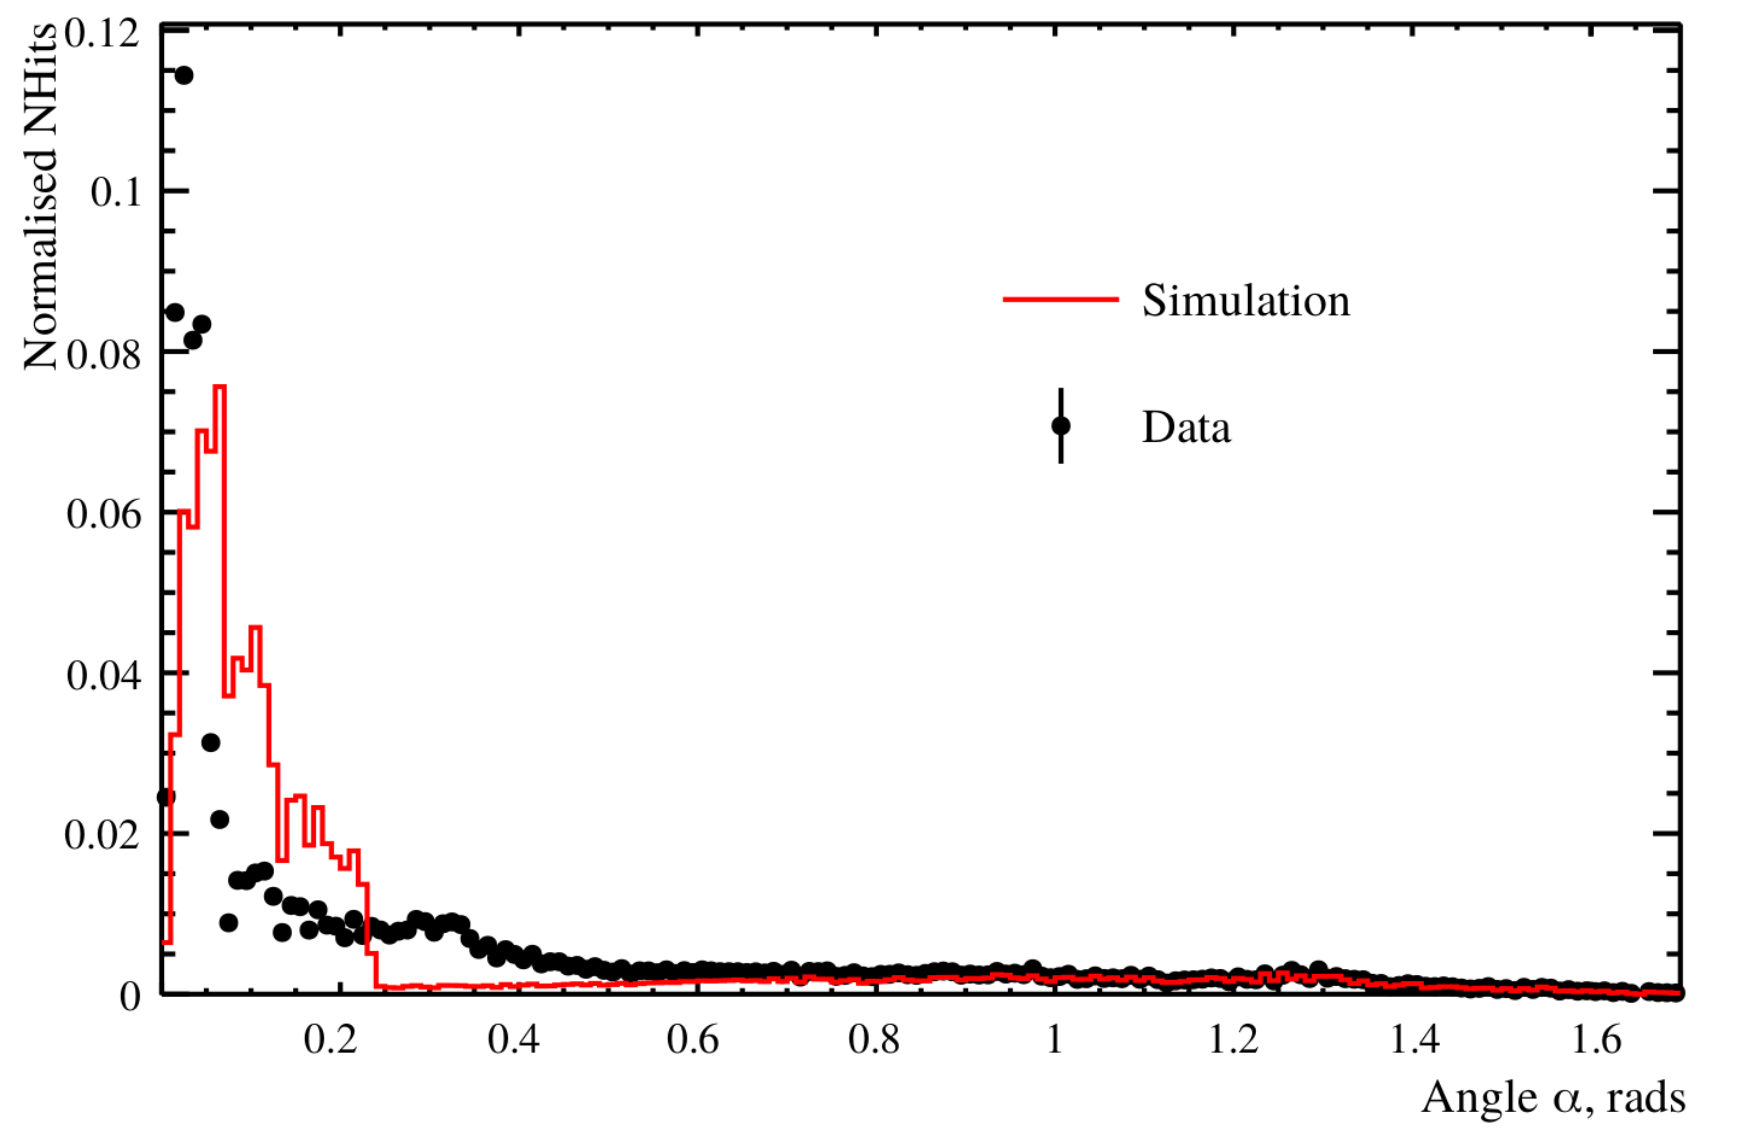
\includegraphics[width=0.7\textwidth]{4_SMELLIESimulation/images/1D_gen_plot.png}
    \caption[Comparison of SMELLIE between data and MC using a 1D generator]{Comparison between a simulation of one of the fibres, made from the 1D beam profile generator (red), with the associated data subrun that was used to create that beam profile (in black). For both MC and data, what is plotted is the PDF of observed PMT hits, as a function of the $\alpha$ angle. Poissonian errors have been added to the data points, but are too small to see. Clearly, this 1D generator does not replicate the observed beam profile correctly. Figure taken from~\cite{turnerMeasurementScatteringCharacteristics2022}.}
    \label{fig:1d_gen_plot}
\end{figure}

This 1D beam profile approach was used initially for SMELLIE, and remains in use for the other ELLIE sub-systems within SNO+. However, when SMELLIE data was taken in the water-phase of the experiment, simulations using these beam profiles failed to match them well at all - see figure~\ref{fig:1d_gen_plot} for an example. Not only was the distribution in $\alpha$ not Gaussian, a distinct speckle-pattern can be observed within the beamspot that is not uniform in $\phi$. This fact led to colleague Esther Turner building a SMELLIE generator that could handle 2D beam profiles: dependent on both $\alpha$ and $\phi$. The distribution was stored as a map from each inward-pointing PMT in the detector to a relative intensity value. This was chosen because the beam profile shapes were calibrated from existing SMELLIE data --- more on this in section~\ref{sect:new_beam_profiles}.

This original 2D generator then sampled the beam profile via a rejection sampling approach, outlined as follows:
\begin{enumerate}
    \item Propose a test direction $(\alpha, \phi)$, by generating $\phi$ uniformly in the interval $[0, 2\pi]$, and $\alpha$ according to some pre-determined Gaussian distribution, known as the Gaussian envelope.
    \item Given this test direction, calculate where a line following this direction from the fibre of interest will hit the PSUP on the other side of the detector. Find the 3 closest PMTs to that point.
    \item From those PMTs, obtain their relative intensity values from the beam profile mapping, and perform an interpolation based on how close each PMT is to the PSUP intersection point. This gives an interpolated relative intensity value for this test direction.
    \item Because we are sampling using the angular coordinates $(\alpha, \phi)$, differential area elements over this space of directions do not have the same size. We can correct for this fact by multiplying our interpolated relative intensity by $\sin{\alpha}$, which corresponds to the Jacobian of the direction-space.
    \item Calculate the value for the Gaussian envelope along this test direction.
    \item Throw a random number uniformly between 0 and the Gaussian envelope value. If the random number is less than the interpolated intensity, then this test direction is accepted, and a photon is generated with that direction. Otherwise, we reject the direction and try the whole process again.
\end{enumerate}

This generator certainly works, but has a key problem: efficiency. The 1D generator was able to generate a SMELLIE event (that is, to fully specify the starting parameters of all the photons emitted from a fibre) at a speed of $\sim\SI{1}{\milli\second}$. However, the 2D generator specified here could take upwards of $\sim\SI{50}{\second}$ \textit{per event} to generate. Because a typical SMELLIE analysis requires simulating many millions of events, the CPU time taken to perform this quickly became unfeasible. Fixing this generator speed problem was a high priority for the SMELLIE analysis.

\subsection{The new generator}\label{sect:new_gen}
On careful inspection of the existing 2D generator, the main reason for the slowness of the algorithm is the use of a rejection approach. Even with use of the Gaussian envelope, which was included to help with speed, the vast majority of proposed directions are never selected. Figure~\ref{fig:num_attempts} shows a histogram of number of attempts per event it took for a valid direction to be chosen for a representative SMELLIE simulation. Moreover, the calculations needing to be done for every proposed direction are relatively complex, notably trying to find the 3 nearest PMTs to some point on the PSUP.

\begin{figure}
    \centering
    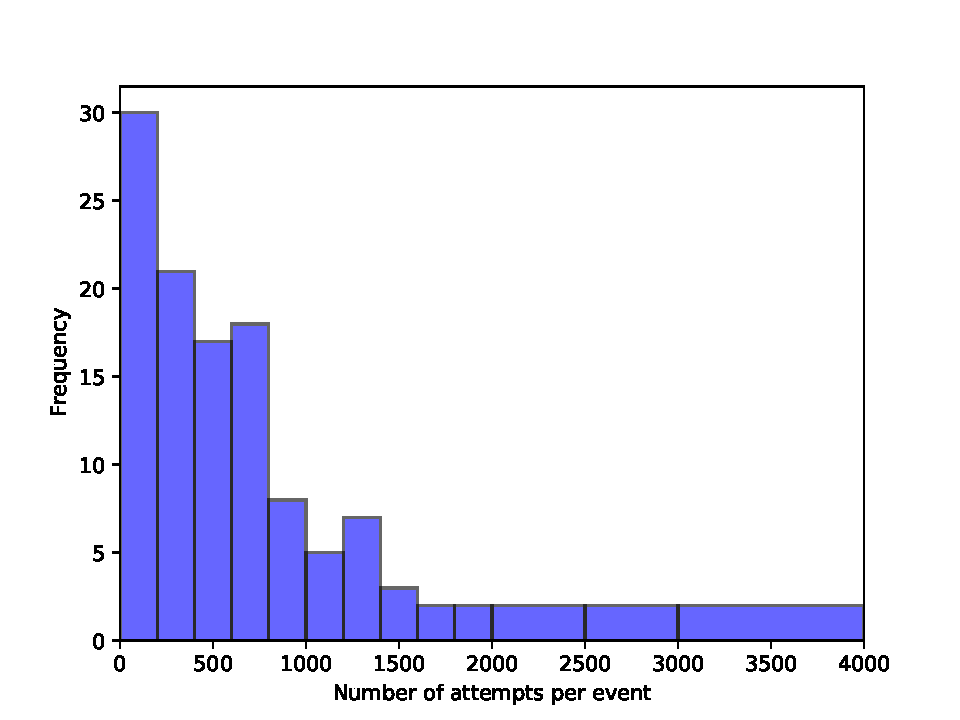
\includegraphics[width=0.7\textwidth]{4_SMELLIESimulation/images/2D_generator_num_attempts_nicer.pdf}
    \caption[Number of attempts taken for existing 2D SMELLIE generator to accept direction]{Typical distribution of the number of attempts it takes for the existing 2D generator before the test direction gets accepted, per event.}
    \label{fig:num_attempts}
\end{figure}

A new 2D generator was built with these thoughts in mind. Firstly, the rejection method would no longer be used, given its inefficiency. We would also endeavour to try and ``pre-calculate'' as much as possible before run-time. Starting with the existing PMT relative intensity maps, we plot these in the 2D direction-space $(1-\cos\alpha, \phi)$: see Figure~\ref{fig:esther_beam_profile}. In a toy-MC simulation, \num{500000} directions are then thrown uniformly in this 2D space per fibre. For each direction, the same method of obtaining an interpolated intensity value from the nearest PMTs to the corresponding point on the PSUP as from the original 2D generator was performed, the only difference being that these calculations were done well before any actual SMELLIE simulation. Figure~\ref{fig:old_profile_interpolated_sample_plot} shows the interpolated intensities obtained for one fibre.

\begin{figure}
    \centering
    \begin{subfigure}{0.98\textwidth}
        \centering
        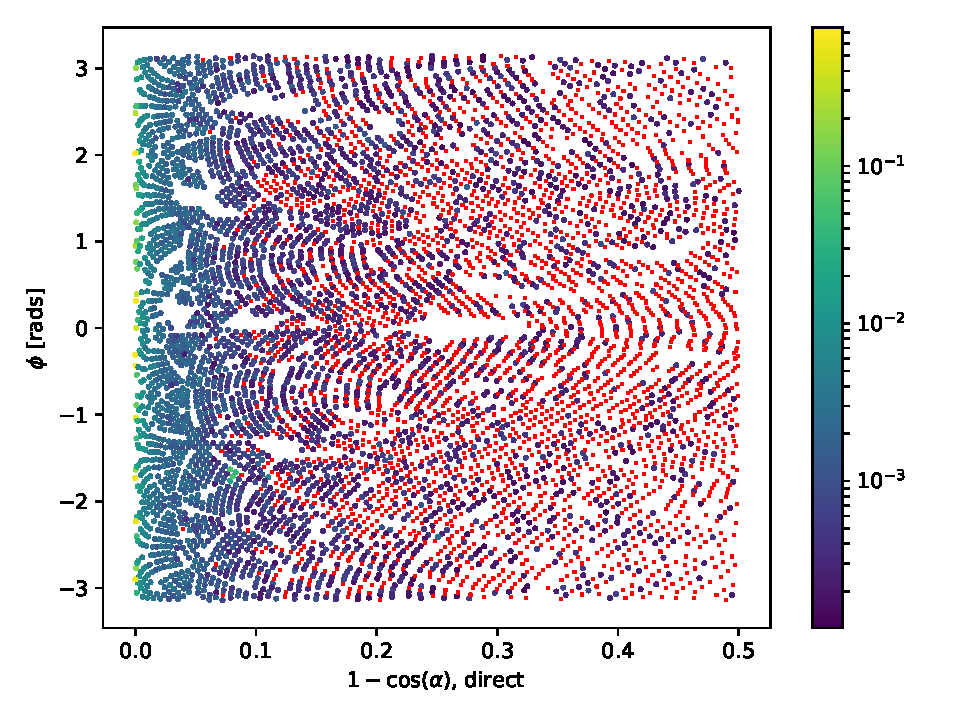
\includegraphics[width=0.74\textwidth]{4_SMELLIESimulation/images/flat_plot_r_FS055_beam_profile_original_6-18-13.pdf}
        \caption{PMT relative intensity map}
        \label{fig:esther_beam_profile}
    \end{subfigure}
    \begin{subfigure}{0.98\textwidth}
        \centering
        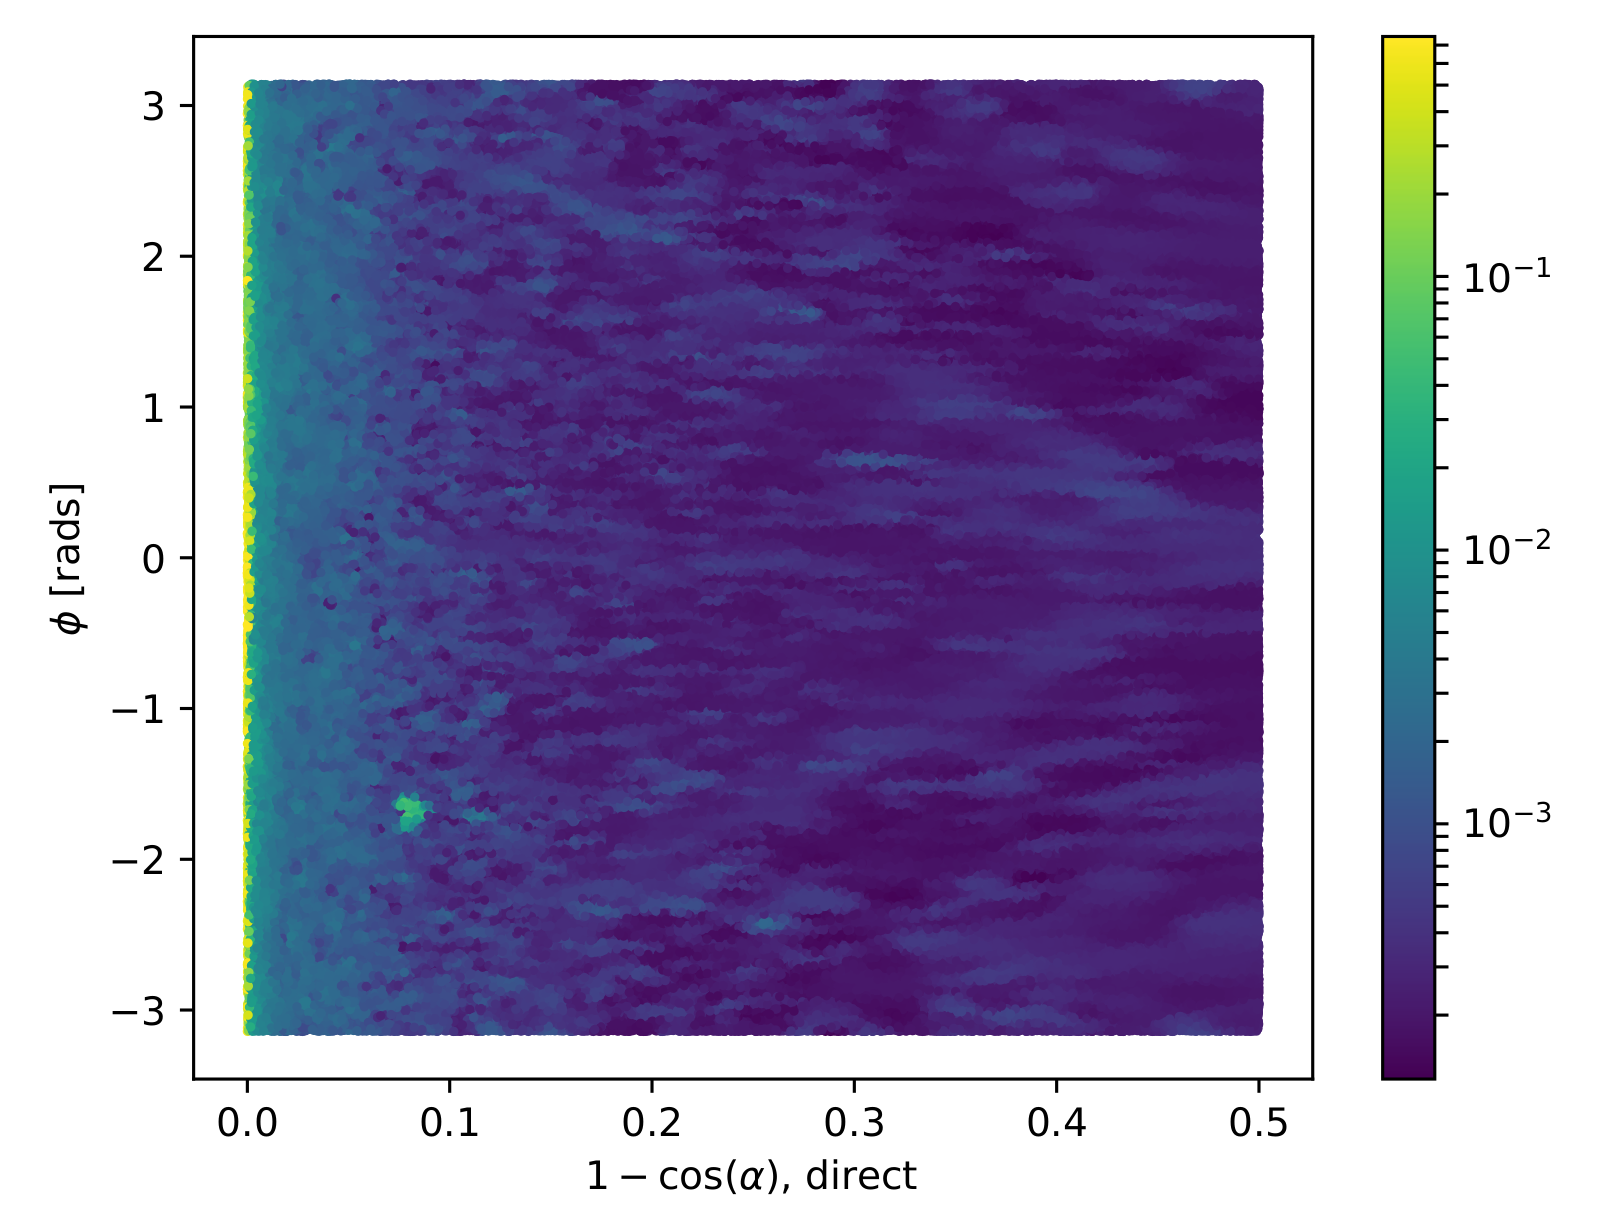
\includegraphics[width=0.74\textwidth]{4_SMELLIESimulation/images/polar_plot_FS055_MC_sampling_old_beam_profile.png}
        \caption{Interpolated intensity map}
        \label{fig:old_profile_interpolated_sample_plot}
    \end{subfigure}
    \caption[Intensity map of existing beam profile, and interpolated sampling map]{The first step in the new method for preparing the new generator. In (a), the relative intensities used for the existing beam profile of fibre labelled FS055 are shown for each PMT, the position on the plot indicating the location of that PMT in the fibre coordinates. The colour indicates the relative intensity; PMTs marked red have an intensity of zero. Figure (b) shows the result of throwing \num{500000} directions uniformly over this 2D space, the intensity of each point given by interpolating the intensities of nearby PMTs.}
    \label{fig:esther_beam_profile_and_interp}
\end{figure}

Following this, the sampled intensities were then binned into a 2D histogram, where the bin value corresponds to the sum of all intensities for all directions found within this bin. Choosing a sensible binning procedure is important: too few bins, and necessary information about the shape of the beam is lost, whilst too many bins can oversample the data and capture statistical artefacts in the sampling process instead of just the beam profile. As a balance, 15 bins were chosen along the $\phi$ direction, and 60 in $r=1-\cos\alpha$. This was chosen to ensure that a reasonable number of PMTs were located within each bin, lessening the impact of any statistical fluctuations. Although the bins in $\phi$ were chosen to have uniform width, this was decided to be not the case for the other axis, as there is far more important information near $r = 0$ (the beamspot). Instead, the width of the bins in $r$ were calculated so that roughly the same total probability was contained in each $r$-strip. By consequence, bins near the beamspot typically are of significantly smaller size than ones much further out. This allows us to both capture any rapid changes in intensity near the beamspot, where this matters greatly, and smooth out the very-low intensities seen at larger polar angles. One of these histograms can be seen in Figure~\ref{fig:hist_cdf_old_profile}: the large change in bin widths as a function of $r$ is clear. One can also see that near the beamspot notable dependence on the intensity as a function of $\phi$. The mysterious ``spot'' at $r = 0.08$, well out of the beamspot, is an indication that the underlying beam profile data being used requires improvement: more on this in section~\ref{sect:new_beam_profiles}.

\begin{figure}
    \centering
    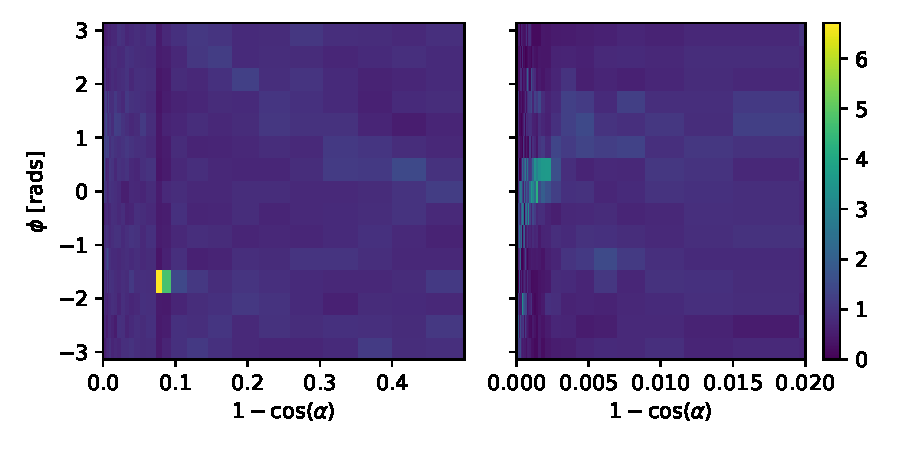
\includegraphics[width=\linewidth]{4_SMELLIESimulation/images/FS055_60_alpha_15_phi_hist.pdf}
    \caption[Histogram of interpolated intensities within the 2D direction-space]{Histogram of interpolated intensities within the 2D direction-space. The left view shows the full histogram; the right is a zoomed-in version near the beamspot. Unlike the binning in $\phi$, the bin widths in $r$ are not at all uniform. Instead, they have been determined such that the area summed over a given ``strip" of bins of constant $r$ will be the same.}
    \label{fig:hist_cdf_old_profile}
\end{figure}

\nomenclature{\textbf{CDF}}{Cumulative Density Function}
The Cumulative Density Function (CDF) of this intensity histogram as a function of bin was then produced, where the bins were ordered through a raster-scan: scanning first over $\phi$, and then $r$. The CDF was then normalised to 1 so that it was well-defined. It is this CDF object that is then loaded in and sampled from during event generation. To do this, an ``inverse-CDF'' approach was used, which has the major benefit over rejection sampling of always producing a valid direction for every sample made. The algorithm works as follows:

\begin{enumerate}
    \item Throw a random number uniformly in $[0,1]$.
    \item Perform a binary search to find the bin that has the largest CDF value below this random number.
    \item Look at the bin edges in $\phi$ of this selected bin: use linear interpolation of the random number to obtain a $\phi$ value located between these two $\phi$-values.
    \item Look at the selected bin's $r$-bin edges, and select a value of $r$ by throwing a second random number uniformly between the two edges. Convert this $r$ into a polar angle $\alpha$.
    \item The photon's direction is defined by the $(\alpha, \phi)$ chosen by this process. 
\end{enumerate}

Because of the relative simplicity of this algorithm compared to the previous 2D generator, the speed improvement was very large: generation now took $\sim\SI{1}{\milli\second}$ per SMELLIE event, a speed improvement of nearly $\num{50000}$. Event generation became as fast as it was when the 1D generator was being used. Furthermore, because of the approach taken, this major speed improvement comes at no sacrifice in accuracy. Figure~\ref{fig:data_generator_comp_new_profiles} shows a comparison of the average number of photoelectrons (npe) per event per PMT between water-phase SMELLIE data and simulations with both the old and new 2D generator. One can see clearly that both generators are as accurate as one another. Note that this plot uses the updated beam profiles as explained in the next section.

\begin{figure}
    \centering
    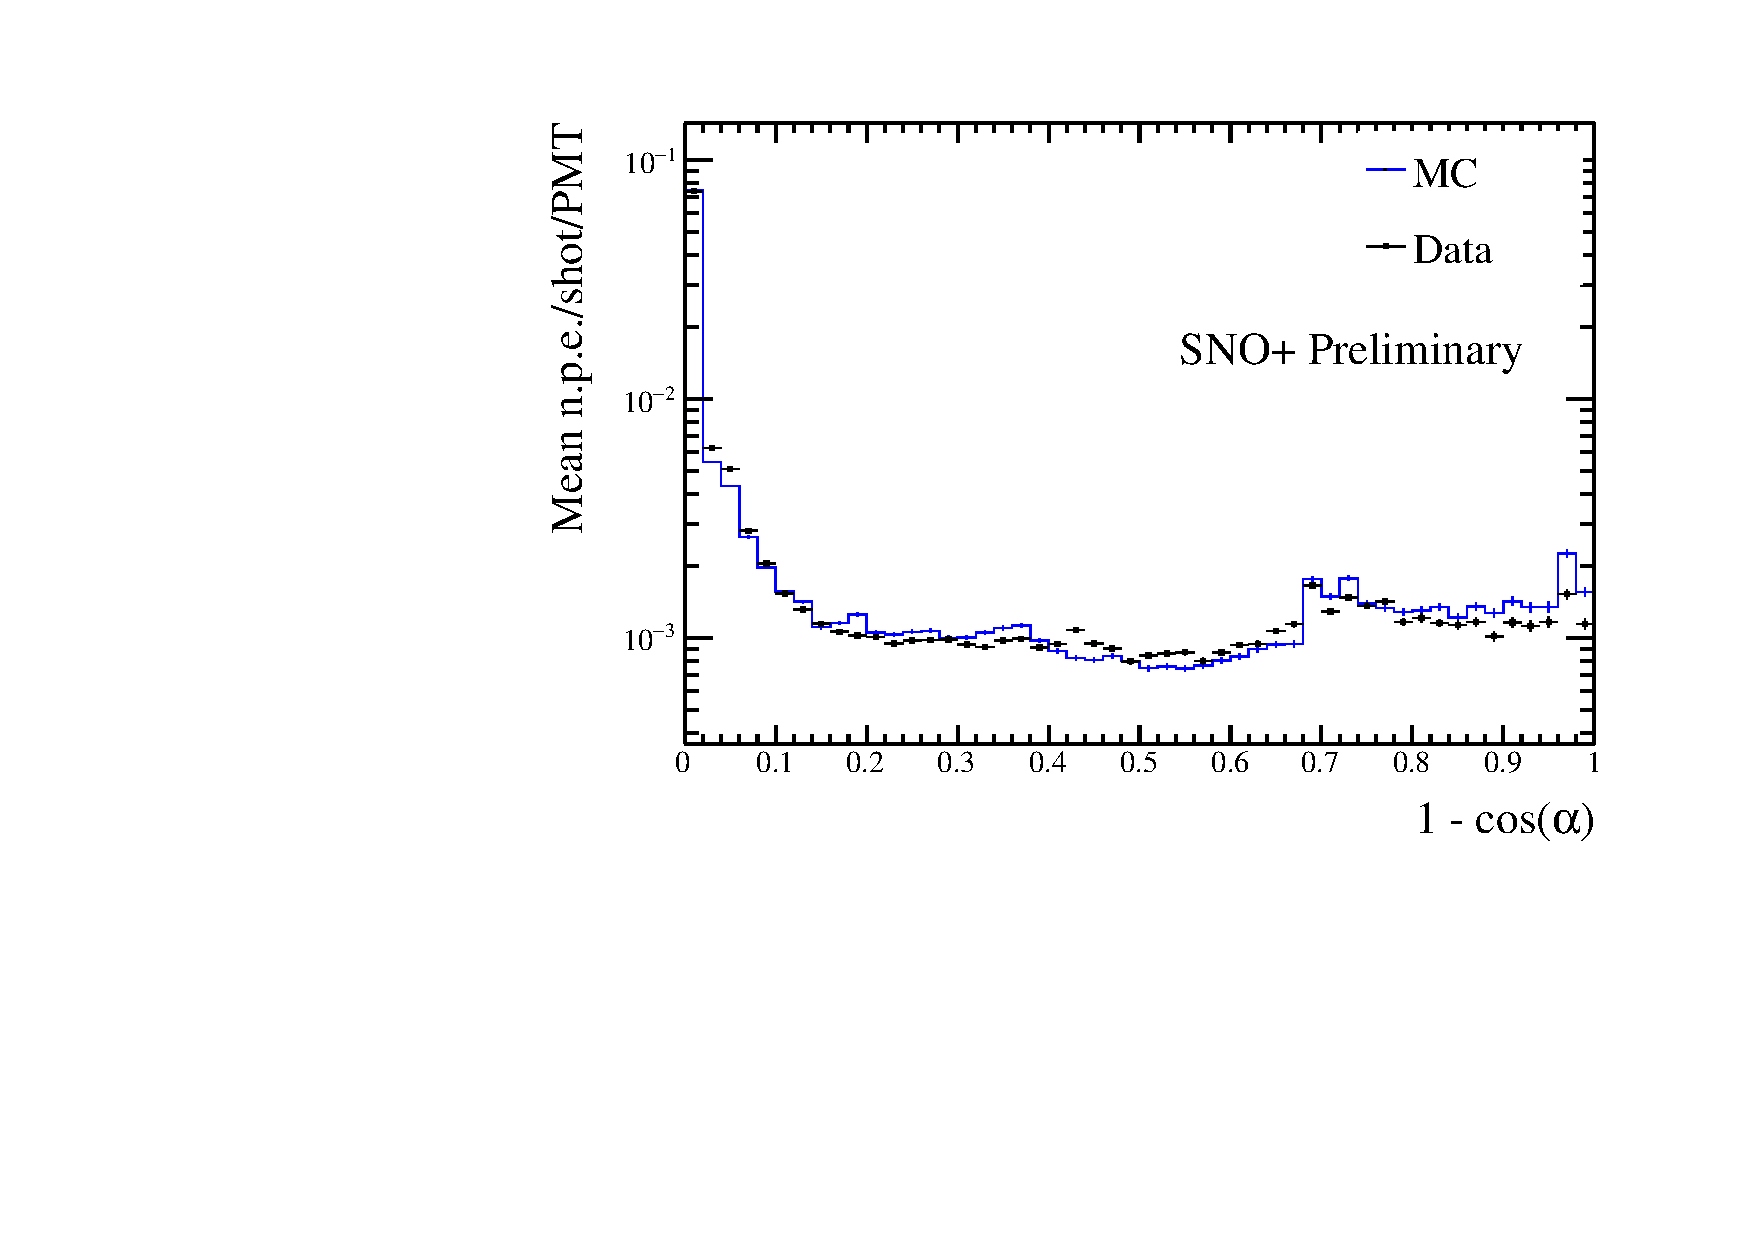
\includegraphics[width=\linewidth]{4_SMELLIESimulation/images/data_mc_comparison_npe_vs_r_114018_109_use_f.pdf}
    \caption[Comparison of water-phase data to MC generated using both the old and new 2D beam profile generator approaches, with the updated beam profiles]{Comparison of water-phase data to MC generated using both the old and new 2D beam profile generator approaches, with the updated beam profiles. Both versions of the generator are consistent with one another, but the new generator is many times faster.}
    \label{fig:data_generator_comp_new_profiles}
\end{figure}

\section{Improving the beam profiles}\label{sect:new_beam_profiles}
Even with the new 2D profile generator, a problem remains: the simulation fails to reasonably recreate data, and much of this appears to be because of the poor beam profile data being used. The curious ``spot'' for one of the fibres was already noted in the previous section that doesn't seem to be physical, and more broadly at large angles for all the fibres there are large swathes of PMTs with an intensity of zero, providing little useful information about the beam shape. It was shown in~\cite{turnerMeasurementScatteringCharacteristics2022} that with the old 2D generator, the systematic uncertainty on the beam profiles was the dominant source of error in the main SMELLIE analysis. To help improve this situation, it was decided to update the existing beam profiles.

These old beam profiles were originally determined by looking at SMELLIE data taken during the water-phase. Specifically, a ``medium''-intensity subrun with one of the lasers firing at a wavelength of \SI{495}{\nano\metre}, was chosen for each fibre. ``Medium''-intensity corresponds to firing the relevant laser at a set intensity determined during an earlier commissioning process, for which the maximum occupancy of PMT hits at that intensity, i.e. the proportion of hits per event, corresponded to roughly 80\%. This value was chosen as it allowed for high statistics in a relatively short run-time, but not so intense that the occupancy of any given PMT in the beamspot was 100\%. Because Rayleigh scattering is strongly-dependent on wavelength, the long wavelength of light was chosen so that impacts from this scattering were small in the data.

SNO+ PMTs are unable to distinguish the exact number of photoelectrons being generated. One is typically only able to know if a PMT has been triggered at all, by any number of photoelectrons. As a result, the occupancy of a PMT over a number of SMELLIE events, $o$, is a biased estimator of the mean number of photoelectrons generated, $\mu$. Assuming the number of photoelectrons generated in a given event follows Poisson statistics, the probability of generating $k$ photoelectrons is:

\begin{equation}
    P\left(k | \mu\right) = \frac{\mu^{k}e^{-\mu}}{k!}.
\end{equation}

The probability of observing a ``hit'' in a given PMT corresponds to generating at least one photoelectron:

\begin{equation}\label{eq:p_hit}
    P\left(\text{hit}| \mu\right) = P\left(k\geq 1 | \mu\right) = 1 - P\left(k = 0 | \mu\right) = 1 - e^{-\mu},
\end{equation}
which implies after rearrangement that one can determine the mean number of photoelectrons per event from the occupancy by:
\begin{equation}\label{eq:multihit_correction}
    \mu = \ln\left(1 - o\right).
\end{equation}
This is the reason why we want to avoid PMTs with occupancies of 100\%: they preclude one's ability to convert into a value for $\mu$ by looking at occupancy alone. We call this conversion from occupancy into npe the ``multi-hit correction''. The impact of this correction is typically small for most PMTs, but can become very significant in a fibre's beamspot.

Once the npe mapping from data was obtained, a correction was then made for the detector's optics: even ignoring a fibre's beam profile, we still expect certain PMTs to be illuminated more than others because of e.g. reflections off the AV, or the solid angle subtended by the PMT bucket opening. For each fibre, a simulation was made where the beam profile was set as isotropic, and the corresponding npe mapping obtained: this map held information about the detector optics only. The beam profile mapping was then derived by simply dividing each fibre's npe mapping from data to its associated isotropic MC npe map. It is these maps that were first used in section~\ref{sect:new_gen}.

\subsection{Combining beam profile datasets}\label{sec:combining_beam_profiles}
% \begin{center}
    \begin{table}
        \begin{tabular}{c p{6cm} p{6cm}}
            \hline
            Run Number & Run Type & Comments \\ \hline \hline
            \num{114018} & All PQ lasers; SuperK laser in \SIrange{400}{500}{\nano\metre} range & Only PQ495 laser and SuperK at \SI{495}{\nano\metre} is used \\
            \num{114023} & SuperK laser in \SIrange{500}{600}{\nano\metre} range & Part 1 of this wavelength range; crash occurred on last subrun, so that subrun is ignored \\
            \num{114034} & SuperK laser in \SIrange{500}{600}{\nano\metre} range & Part 2 of this wavelength range \\
            \hline
        \end{tabular}
        \caption{Water-phase runs used for new beam profiling.}
        \label{tab:runs_used}
    \end{table}
% \end{center}
Fortunately, much more SMELLIE data was taken during the water-phase than was used for the original beam-profiling analysis. This additional data can be combined with that which was already used to far better constrain the beam profiles. In particular, given the existing assumption that scattering effects are minimal above wavelengths of $\sim\SI{490}{\nano\metre}$, all data taken with wavelengths above this can also be used. The specific runs (and associated comments about their specifics) are described in Table~\ref{tab:runs_used}. Because high-intensity runs require a different analysis approach (PMTs with high occupancies must use charge, not occupancy, to  estimate npe), for this analysis we only considered subruns that used low or medium intensity set-points.

For each subrun $j$ of data per fibre, we look only at PMT hits for each PMT $i$ that has been identified as ``good'' for that subrun\footnote{Strictly speaking, a PMT's ``goodness'' is only determined on a run-by-run, not a subrun-by-subrun level, but this has no impact on the analysis.}, $i \in G_{j}$. $G_{j}$ here represents the set of good PMTs in subrun $j$. In particular, a ``good'' PMT must have valid electronic and timing calibrations, be at high voltage and masked into the detector's trigger system for that subrun. In addition, an angular cut of $\alpha < \SI{60}{\degree}$ was made to remove PMTs that are well outside any reasonable beam direction. To isolates the hits arriving directly from the fibre without reflecting, scattering, or being noise, a time cut was also made. Because what matters is the time relative to emission from the fibre, and the expected time-of-flight from fibre to different PMTs varies, a quantity known as the time residual was used. Starting with the calibrated hit time of a given PMT relative to the event's trigger time, $t_{hit}$, the expected time-of-flight $t_{TOF}$ from the fibre to the PMT was subtracted, estimated with the collaboration's ``Light Path Calculator''. Then, the emission time was also subtracted, $t_{emm}$, estimated by looking at the second-earliest value of $t_{hit}-t_{TOF}$ within the fibre's central beamspot, defined as the PMTs for which $\alpha<\ang{3}$. It was found that a ``loose'' time residual cut of $t_{res} \in [-10, +12] \si[]{\nano\second}$ was sufficient to remove the vast majority of non-direct light with little signal sacrifice. In the situation where a subrun with intensity was very small, it would not regularly have at least two hits in the beamspot, and so the time residuals calculated would not be valid for many events. To avoid this situation, a cut was made on any subruns with mean intensities below 9 within their beamspot. This value was chosen as it would mean a $2\sigma$ fluctuation downwards of $2\cdot\sqrt{9}=2\cdot3=\SI{6}{\npe}$ would still have more than the 2 hits necessary for timing reconstruction. One fibre, FS207, has no data subruns that satisfy this condition, and as such will have to be dealt with separately. For the time being, this fibre was ignored.

Extracting the underlying beam profiles from these data required some careful thought, especially because different subruns could have different intensities. Considering a PMT $i$ in subrun $j$, the mean number of photoelectrons generated per event in that PMT for that subrun, $\mu_{ij}$ can be decomposed as follows:

\begin{equation}\label{eq:mu_def}
    \mu_{ij} = I_{j}k_{i} = I_{j}b_{i}f_{i}.
\end{equation}
$I_{j}$ is the intensity of the subrun, i.e. the mean number of photons generated from the fibre in that subrun per event. $k_{i}$ is the probability that a given photon generated at the fibre source ends up generating a photoelectron in PMT $i$. This itself can be further split into two components: $b_{i}$, the probability that a given photon at the fibre source points in the direction of PMT $i$; and $f_{i}$, the probability that a given correctly-pointed photon actually makes it to the PMT and successfully generates a photoelectron. It is $b_{i}$ that is the actual beam profile we would like to measure.

Letting $p_{ij}$ be the probability of observing a hit for a given event on a given PMT, the probability of observing $m_{ij}$ hits out of $N_{j}$ events in the subrun will be binomially-distributed:
\begin{equation}
    P(m_{ij}| \mu_{ij}) = L(\mu_{ij} | m_{ij}) = \binom{N_{j}}{m_{ij}}p_{ij}^{m_{ij}}(1-p_{ij})^{N_{j}-m_{ij}} = \binom{N_{j}}{m_{ij}}\left(1-e^{-\mu_{ij}}\right)^{m_{ij}}e^{-\mu_{ij}(N_{j}-m_{ij})}.
\end{equation}
Here we have used equation~\ref{eq:p_hit}, and noted that this probability distribution in $m$ can be re-framed as a likelihood function for the parameter $\mu_{ij}$. Considering only a single subrun of data, the maximum likelihood estimate of the parameter $\mu_{ij}$ can be shown to be:
\begin{equation}
    \left<\mu_{ij}\right> = -\ln\left(1-\frac{m_{ij}}{N_{j}}\right) = \ln\left(1-o_{ij}\right) \qquad(m_{ij} \neq N_{j}),
\end{equation}
where $o_{ij}$ is just the occupancy of PMT $i$ in subrun $j$. This is just the multi-hit correction formula seen in equation~\ref{eq:multihit_correction}, which makes sense.

When looking at multiple subruns for the same fibre, the total likelihood function for a given PMT when considering all the data for a given fibre will be the product of the likelihoods from each dataset,
\begin{equation}
    L\left(\left\{I_{j}\right\}, k_{i} | \left\{m_{ij}\right\}\right) = \prod_{j} L(I_{j}, k_{i} | m_{ij}) = \prod_{j}\binom{N_{j}}{m_{ij}}\left(1-e^{-I_{j}k_{i}}\right)^{m_{ij}}e^{-I_{j}k_{i}(N_{j}-m_{ij})}.
\end{equation}
This leads to a log-likelihood distribution of
\begin{equation}
    \mathcal{L}\left(\left\{I_{j}\right\}, k_{i} | \left\{m_{ij}\right\}\right) = \sum_{j}\left[\ln\left(^{N_{j}}C_{m_{ij}}\right) + m_{ij}\ln\left(1 - e^{-I_{j}k_{i}}\right) - I_{j}k_{i}\left(N_{j} - m_{ij}\right)\right].
\end{equation}
Formally, one could combine the likelihoods of all the PMTs together, and by looking at the maximum likelihood estimates for each of the parameters measure the parameter values this way. However, the set of equations one obtains through this approach quickly become analytically intractable, because the PMTs are coupled by the intensity values $I_{j}$. Even a direct numerical approach would be liable to fail: for a given fibre there can be dozens of subruns, and many thousands of PMTs of relevance, so the dimensionality of the system of equations would be far too large.

Because of this, a different approach was taken. It is expected that in a subrun the total npe, summed over all good PMTs, should be proportional to the intensity value $I_{j}$. One must be careful about this construction --- different subruns can have different sets of good PMTs, so two subruns with identical $I_{j}$ values could have a larger summed npe merely because more PMTs were good in that subrun. To counter-act this effect, only PMTs that were classified as good in \textit{all} subruns being analysed for that fibre would be used for the npe summation. In other words, we use data from PMT $i$ for summing only if:
\begin{equation}
    i \in \mathcal{I} = \bigcap_{j}G_{j}.
\end{equation}
We can then define the summed npe for a given subrun as $S_{j} = \sum_{i\in\mathcal{I}}\text{npe}_{ij}$, and assert that $I_{j} = cS_{j}$. By finding a value proportional to $I_{j}$, there is now enough information to maximise the log-likelihood $\mathcal{L}\left(k_{i} | \left\{m_{ij}\right\}, \left\{I_{j}\right\}\right)$ with respect to $k_{i}$ for each PMT independently, and hence obtain estimates for these $k_{i}$ parameters.

Of course, what is actually wanted are the underlying $b_{i}$ values, not $k_{i}$. This is where isotropic simulations come in. For each run of data used, a matching isotropic MC was produced. As an example, a simulation for run \num{114023} contained \num{200000} events for each fibre using an isotropic beam profile, over the full wavelength range considered in this run, \SIrange{500}{600}{\nano\metre}, using the same run conditions as in data (which PMTs were at high voltage, etc.).

For each isotropic MC run, both $I_{j}^{MC}$ and $k_{i}^{MC}$ were calculated via the method described above. Because the simulations were isotropic, the underlying value for $b_{i}$ was constant across all the PMTs, and so $ak_{i}^{MC} = f_{i}$. By doing some rearranging of equation~\ref{eq:mu_def}, we find that:
\begin{equation}
    \mu_{ij} = I_{j}b_{i}f_{i} = cS_{j}b_{i}ak_{i}^{MC} = (acb_{i})S_{j}k_{i}^{MC}.
\end{equation}
As a result of this, given the set $\left\{S_{j}\right\}$ and $k_{i}^{MC}$, one can maximise the log-likelihood $\mathcal{L}$ with respect to $b'_{i} = acb_{i}$ numerically, to obtain the maximum likelihood estimate of $b'_{i}$. Because $a$ and $c$ were global constants of proportionality, they would become irrelevant as soon as the beam profile was normalised in the CDF-creation process outlined in~\ref{sect:new_gen}.

Figure~\ref{fig:likelihood_scan} shows the shape of this log-likelihood distribution for a particular PMT when considering fibre FS007's beam profile. One can see how individual subruns provide much more information when combined than if one looked at a single subrun alone.

\begin{figure}
    \centering
    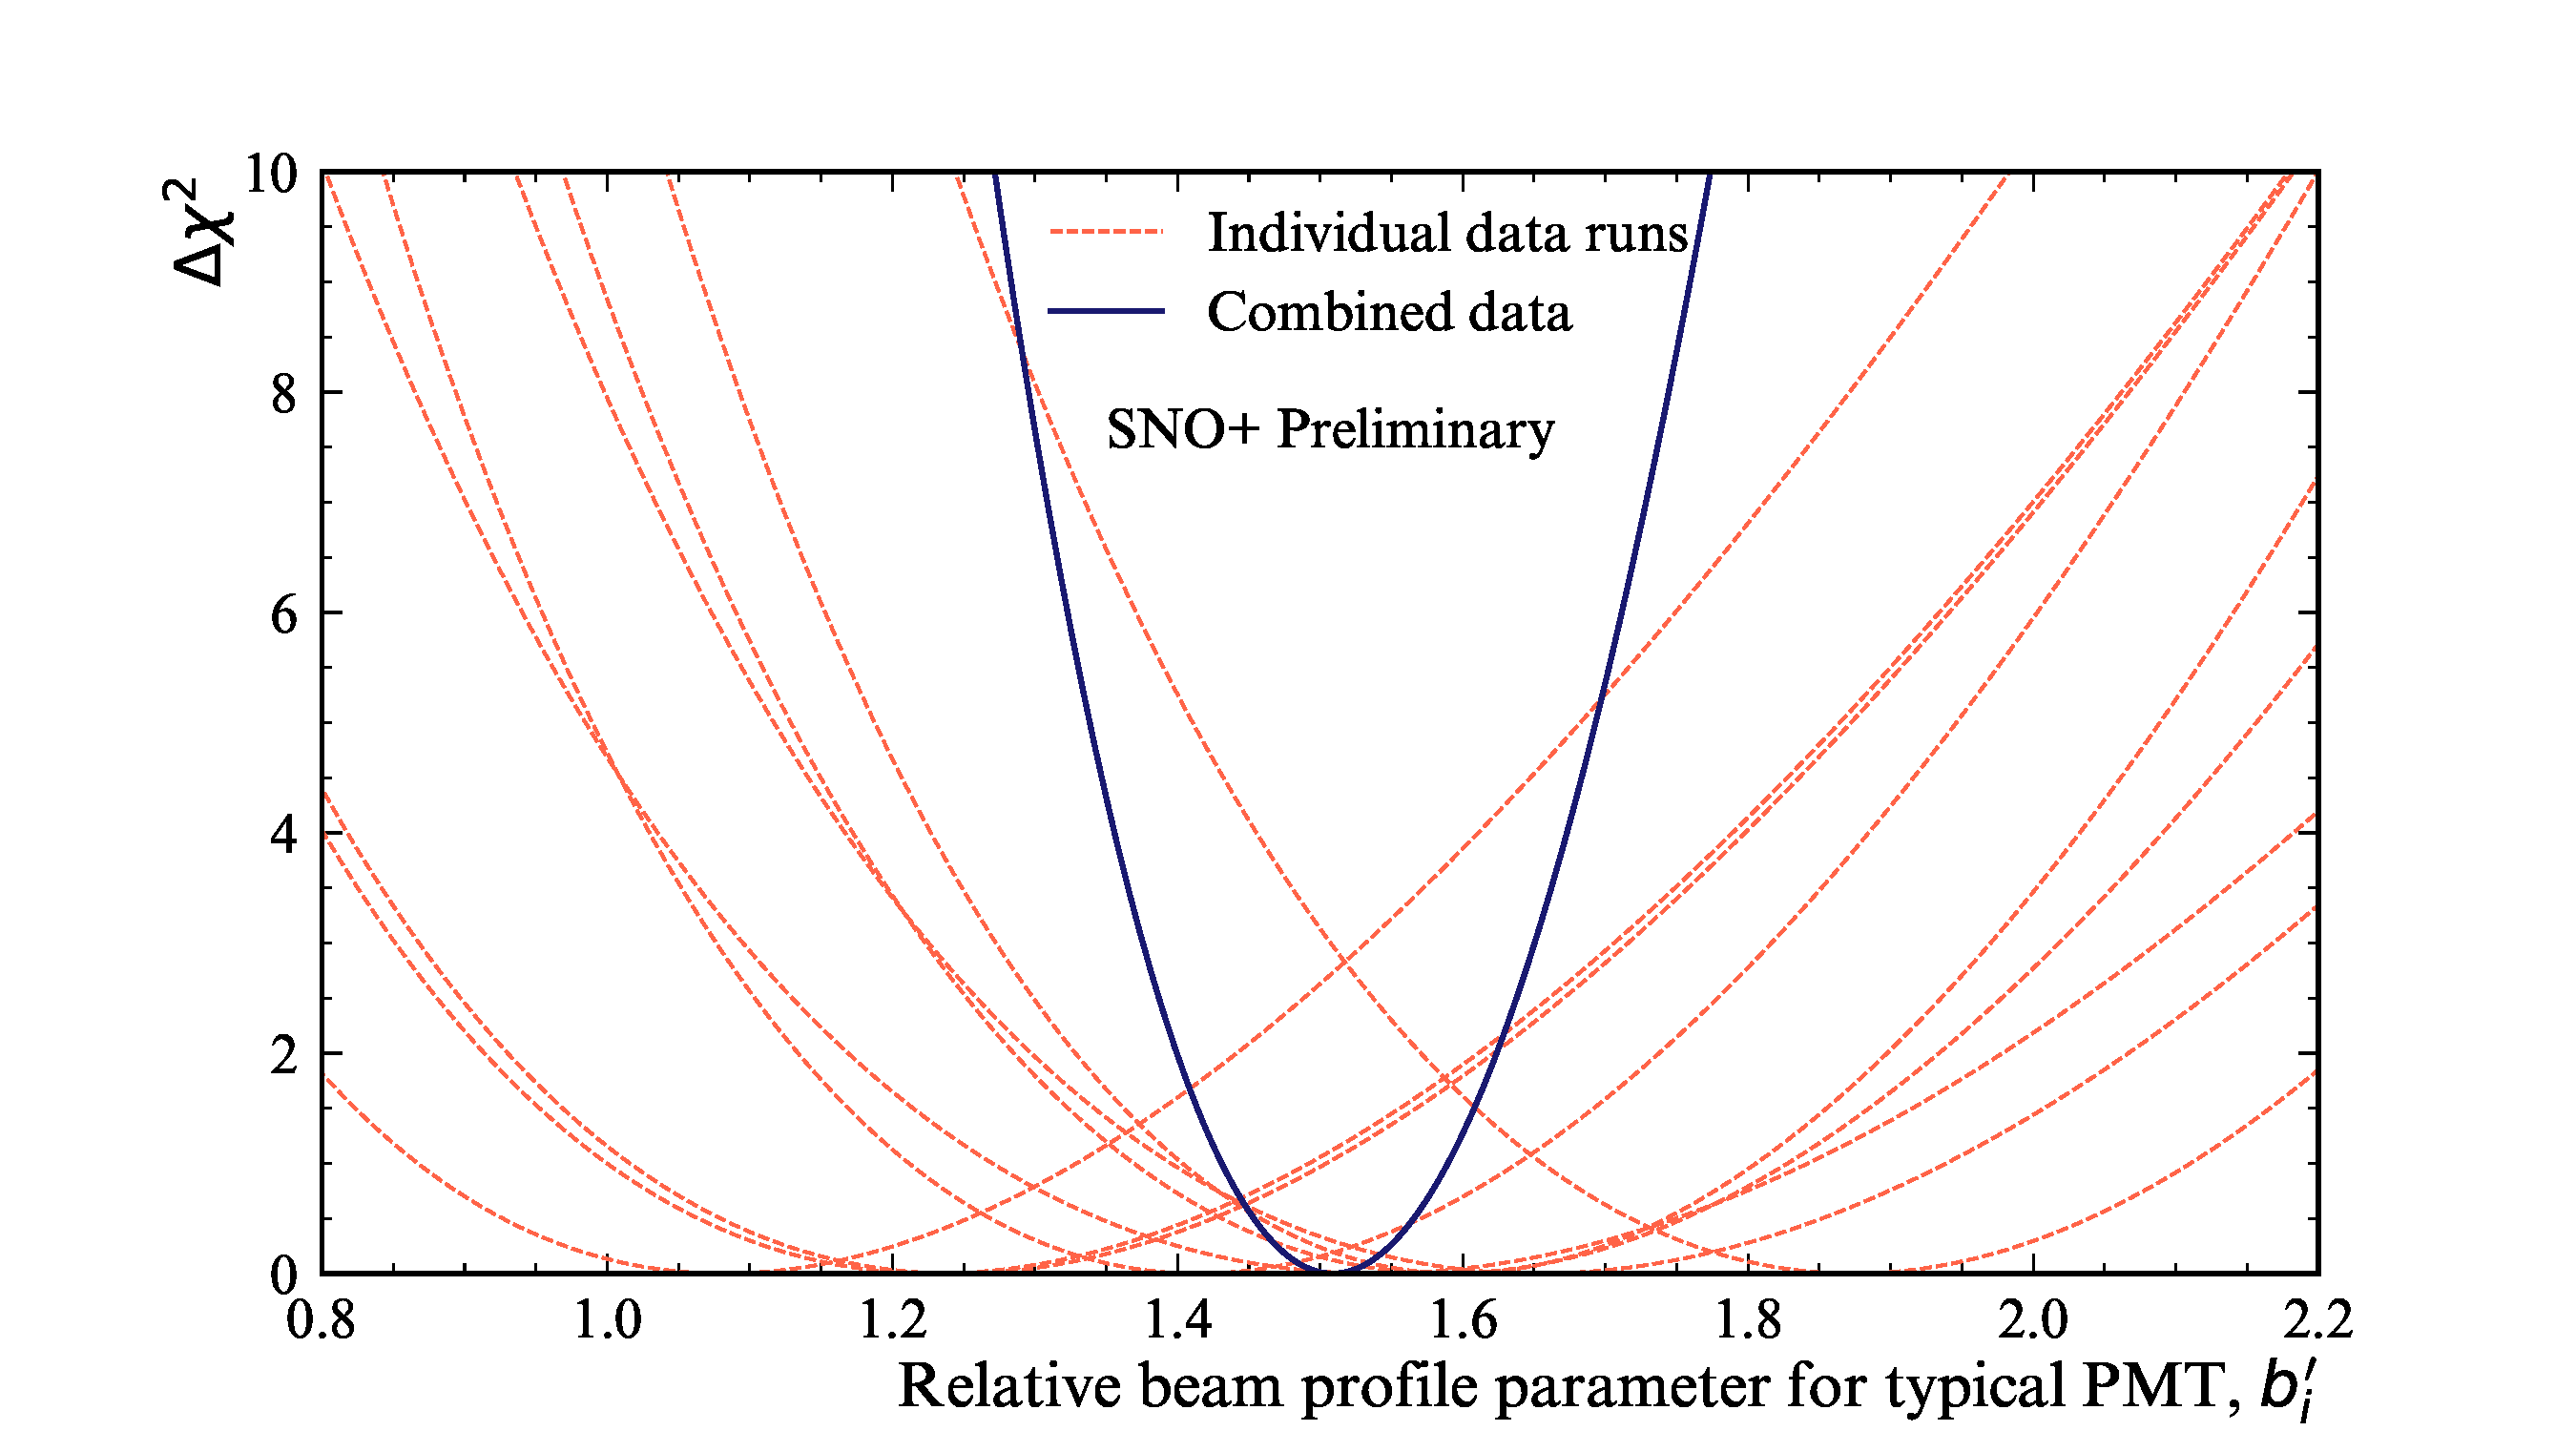
\includegraphics[width=0.8\linewidth]{4_SMELLIESimulation/images/example_likelihood_distribution_pmt_inc_all_subruns_proper_formatting.pdf}
    \caption[Plot of $\Delta\chi^2$ for both single subruns of a typical PMT, and when all relevant subruns are combined]{Plot of $\Delta\chi^2\simeq X_{i}$, twice the negative log-likelihood ratio, for both single subruns of a typical PMT, and when all relevant subruns are combined.}
    \label{fig:likelihood_scan}
\end{figure}

Another benefit of using this log-likelihood approach is that the resulting distribution's shape can be used for uncertainty estimation. In almost all cases, Wilks Theorem~\cite{wilksLargeSampleDistributionLikelihood1938} allows us to produce $1 \sigma$ confidence intervals about the maximum likelihood estimate for $b'_{i}$, $\left<b'_{i}\right>$, because $$X(b'_{i}) = -2\left[\mathcal{L}\left(b'_{i}\right) - \mathcal{L}\left(\left<b'_{i}\right>\right)\right]$$ approximates a $\chi^2$-distribution. As a result, the error bounds on our parameter estimate are given by when $X = 1$. The fact that the shape of $X$ can be well-approximated by a quadratic in the region near $X = 0$ indicates the validity of Wilks' Theorem being used here.

Only a couple of exceptions to this approach of parameter estimation are possible. In the case where $m_{ij} = N_{j}$, i.e. a PMT has 100\% occupancy, no maximum likelihood estimate exists: we need not worry about this, as subruns where this occurs have not been used. On the other end, however, there are some PMTs for certain fibres where after all subruns of data have been included, there remains no hits. In this scenario, one can show that the log-likelihood becomes linear in the beam profile parameter:
\begin{equation}
    \mathcal{L}\left(b'_{i}|\left\{m_{ij}=0\right\}\right) = b'_{i}k_{i}^{MC}\cdot\sum_{j}\left[I_{j}N_{j}\right].
\end{equation}
This scenario is very much reminiscent of rare-decay searches, and a similar approach can be used. A $1 \sigma$ upper limit on the possible value for $b'_{i}$ can be analytically-calculated to be:
\begin{equation}
    b'_{i,ulim} = -\frac{k_{i}^{MC}\sum_{j}\left[I_{j}N_{j}\right]}{\ln\left[1 - \operatorname{erf}\left(1/\sqrt{2}\right)\right]},
\end{equation}
where $\operatorname{erf}(x)$ is the error function.
% {
%     \color{blue}
%     [18 pages for above two sections]
% }

\section{Comparisons between Data and Simulation}\label{sec:smellie_systematics}
In this section, the major systematic differences between simulations of SMELLIE and data that remain after the above improvements have been made are discussed. These fall into three broad categories. The two of these are the differences seen in the forward and back hemispheres of the detector relative to a given fibre; the third are differences in the timing distributions of the light.

\subsection{Forward Hemisphere Discrepancies}\label{sec:smellie_systematics_forward}
Figure~\ref{fig:updated_beam_profile} shows the impact of using additional subruns of data on a typical beam profile. One can clearly see the great reduction in the number of PMTs with no hits in data. That many more data sets were included allowed for the major increase in dynamic range available for measuring these $b'_{i}$ values. One can also note that by including additional data the curious spot that was seen in the old beam profile our at $r\approx0.08$ has gone, further indicating that it was an artefact of that single data set.
\begin{figure}
    \centering
    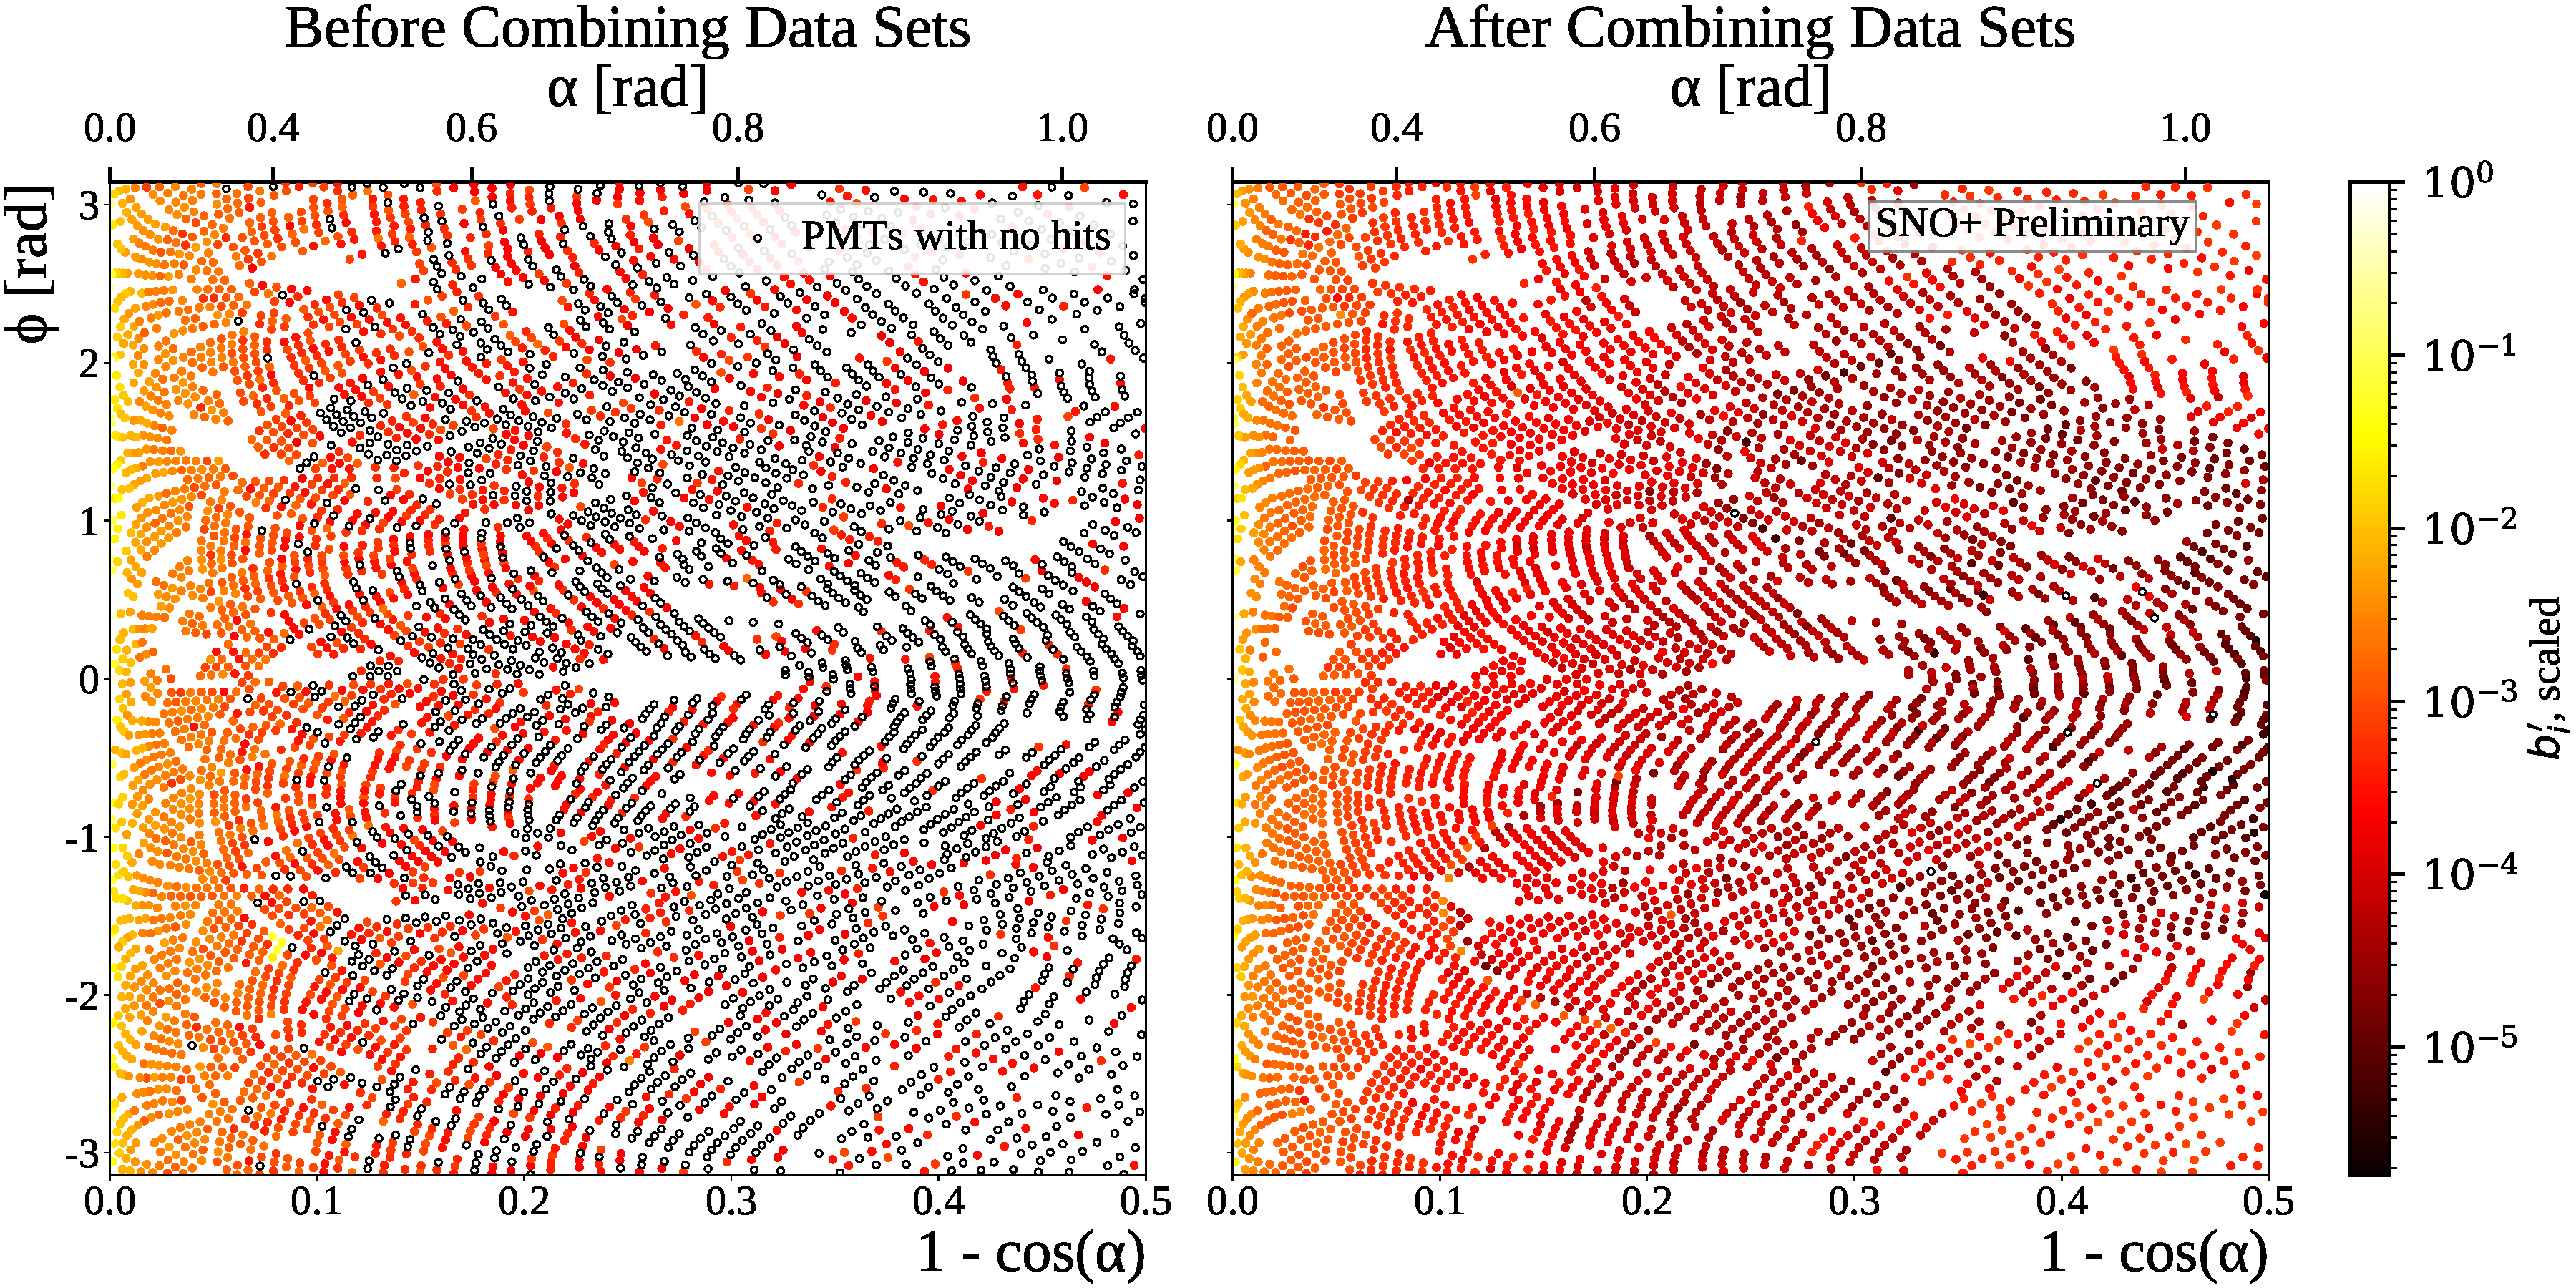
\includegraphics[width=\textwidth]{4_SMELLIESimulation/images/flat_plot_r_comparison_FS055_old_vs_new_empty_circles.pdf}
    \caption[Comparison between old and updated beam profiles for fibre FS055, after combining multiple data sets]{Comparison between old and updated beam profiles for fibre FS055, after combining multiple data sets. Once again, the relative intensities ($b'_{i}$) for each PMT are given by the colour of each point, the position of each plotted in the 2D $(r,\phi)$-space. The relative intensities have been both scaled here so that the largest value equals 1. Hollowed-out points are PMTs that, even after all relevant subruns have been combined, have no PMT hits.}
    \label{fig:updated_beam_profile}
\end{figure}

Further details can be gathered from the interpolated intensity maps, one of which can be seen in figure~\ref{fig:updated_beam_profile_sampling}. There are two curious stand-out features that can be seen here: firstly, there are multiple distinct parabolic arcs. These correspond to the shadows of the ropes that hold up/down the AV. More precisely, they are the mismodelling of those shadows --- if the shadows were in the right place in the isotropic MC, then they would correctly cancel out any decreased intensity seen in the data of shadowed PMTs. These shadows could be mismodelled either because the positions of the ropes in the MC are in the wrong place, or the fibre's emission position is wrong. Note that any mismodelling of the fibre's nominal emission direction has no impact on this shadowing problem, as changing that direction merely causes a change of basis in the $(r,\phi)$-space. The latter possibility of incorrect fibre positions are more likely, and in fact these arcs in the beam profiles could be used as an effective way to correct for this problem.

\begin{figure}
    \centering
    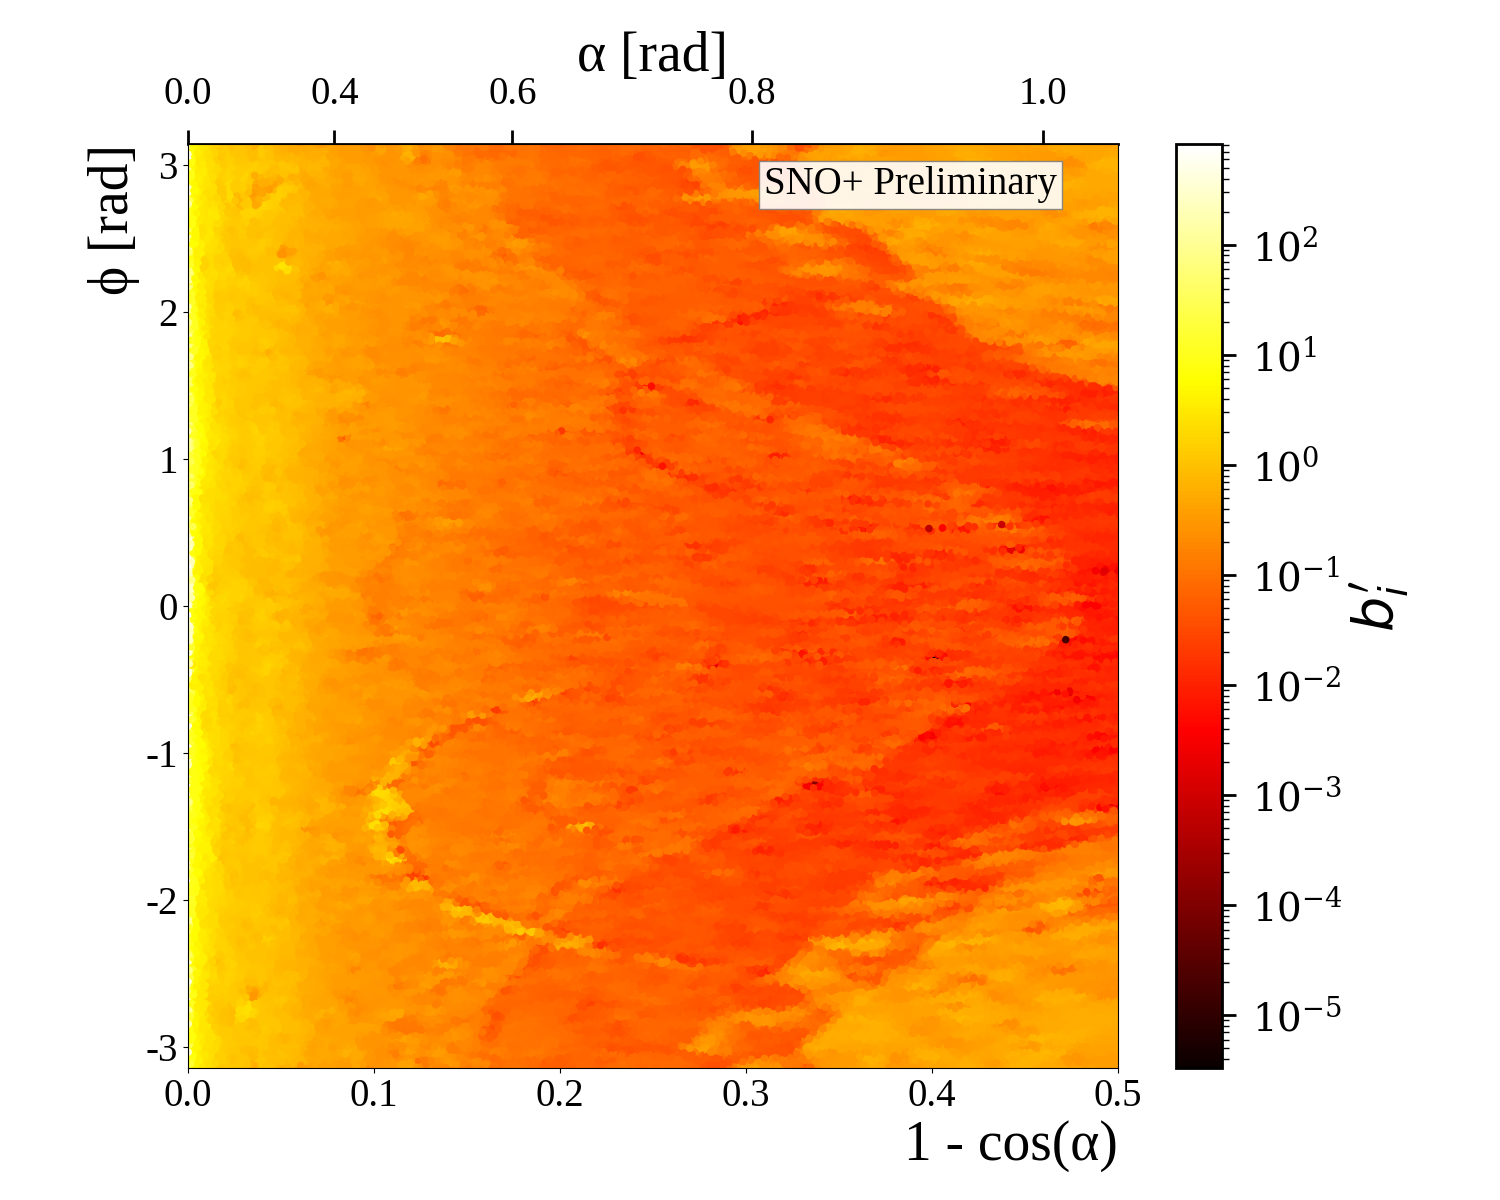
\includegraphics[width=0.8\textwidth]{4_SMELLIESimulation/images/flat_plot_r_FS055_500k_interpolated_beam_profile_full_formatting.png}
    \caption[Interpolated intensity map for the new updated beam profile of fibre FS055]{Interpolated intensity map for the new updated beam profile of fibre FS055. The misalignment of rope shadows and AV effects, can both be seen.}
    \label{fig:updated_beam_profile_sampling}
\end{figure}
The second distinctive feature of this intensity map is the large band of lower intensity varying between $r\approx0.2-0.5$, followed by larger intensity out at large $r$ values. This feature comes from light reflecting off the AV surface, or internally-reflecting. The reason for this band's functional dependence on $\phi$ is that this particular fibre, FS055, has a nominal fibre direction $\sim\ang{10}$ from pointing radially-towards the detector's centre. This feature appears in the updated beam profiles of all fibres, but its shape depends on the particular fibre's direction --- for fibres pointing directly towards the detector's centre, there is little $\phi$-dependence observed. Like the ropes, this feature must come from some form of mismodelling of the optics of the AV. A de-facto shadowing of PMTs in line with tangents from the AV surface which intersect the fibre position is to be expected. One also expects PMTs at polar angles larger than this to have their observed intensities boosted from reflected light off the AV. However, the discontinuities seen in the beam profiles indicate that for whatever reason this effect has been over-emphasised in the simulation.

There is a further phenomenon that can be seen, by comparing beam profile values obtained from a single subrun to the updated combined beam profile. This can be done by calculating the residuals corresponding to the single subrun, relative to the combined data set. The residual is negative if the combined data sets have a $b'_{i}$ below the equivalent for a given single subrun; that is, the combined model underestimates this subrun for that PMT.

This information was plotted for two different subruns from the same fibre, seen in figure~\ref{fig:llr}. One subrun was the same one used by Esther Turner for the original 2D beam profiling, with a wavelength of \SI{495}{\nano\metre}; the latter was at the longer wavelength of \SI{595}{\nano\metre}. For both subruns, most PMTs are seen to have intensities well-modelled by the combined model. However, their appears to be a significant amount of mismodelling within the beamspot. There also appears to be some systematic shift between data and model at somewhat larger polar angles. Moreover, this mismodelling seems not to be merely random, but a function of wavelength: at shorter wavelengths the beamspot tends towards being overestimated and then underestimated at larger values of $\alpha$. At longer wavelengths, the beamspot becomes underestimated, with larger angles getting overestimated. This indicates that there appears to be a wavelength-dependence on the beam profiles, contradicting one of the main assumptions which we used to combine the water-phase data in the first place!
\begin{figure}
    \centering
    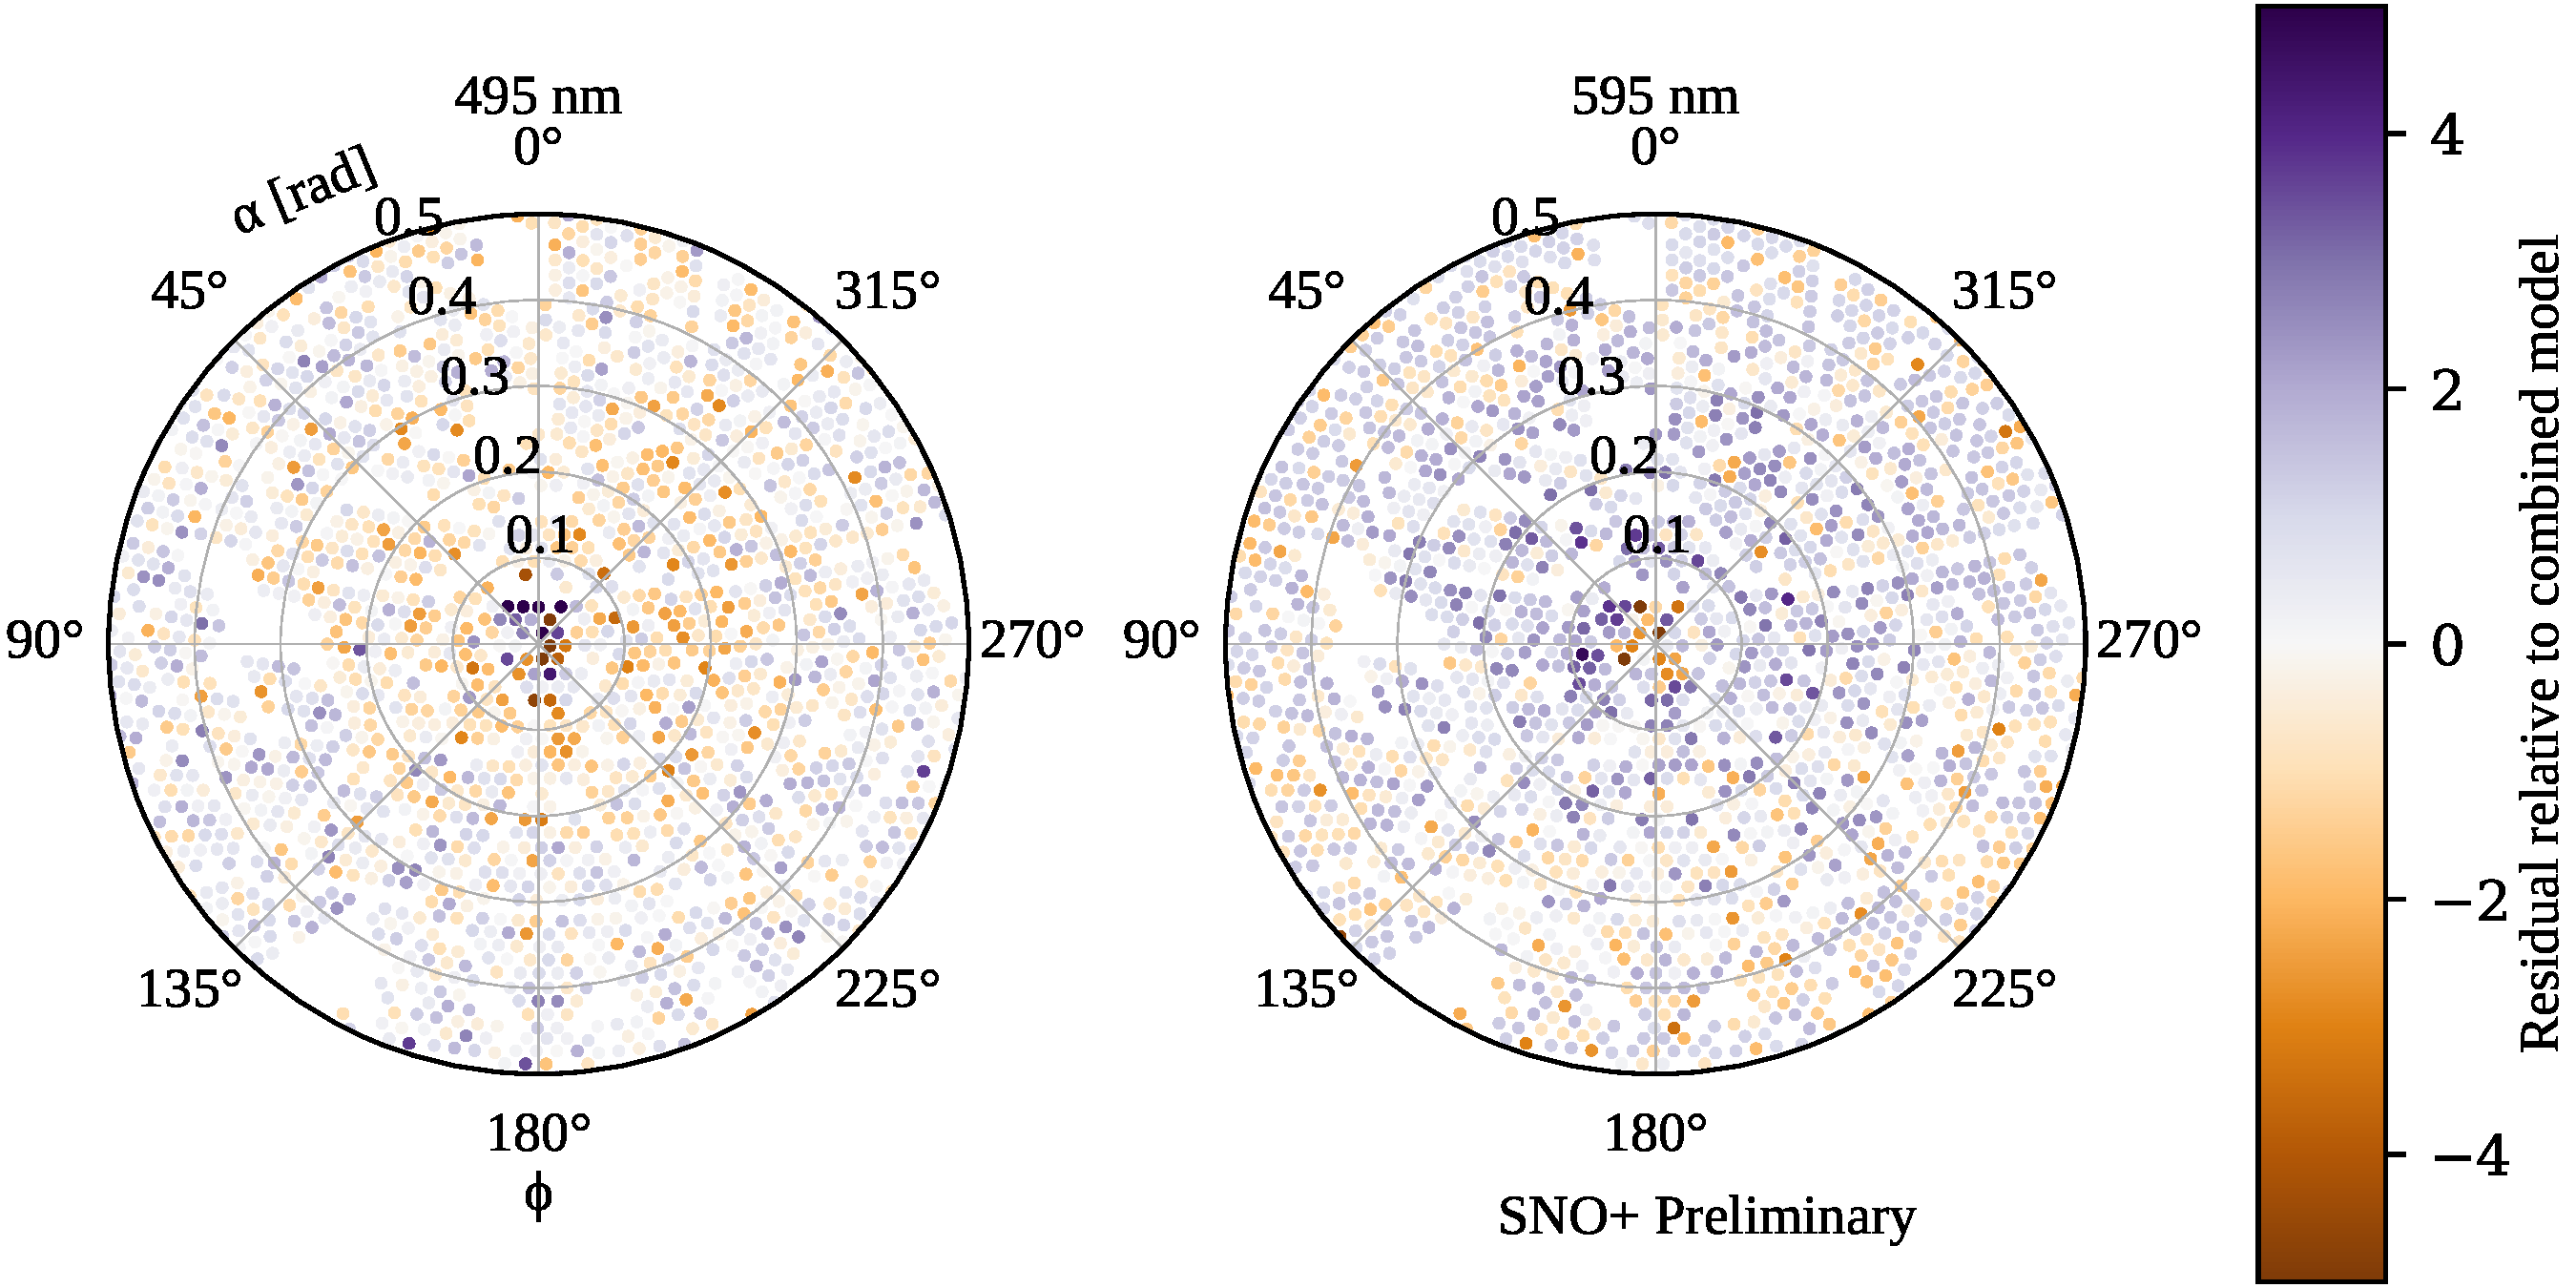
\includegraphics[width=\textwidth]{4_SMELLIESimulation/images/residual_wavelength_comparison_data_model_nice.pdf}
    \caption[Residuals from subruns at two different wavelengths, both compared to the combined beam profile model for fibre FS055]{Residuals from subruns at two different wavelengths, both compared to the combined beam profile model for fibre FS055. A negative sign, and hence bluer colours, indicate that the combined model underestimates the observed intensity for that particular subrun. Values with a magnitude beyond 5 are shown capped at this maximal value for the purposes of this plot. These PMTs are plotted in the polar fibre coordinates $(\alpha,\phi)$.}
    \label{fig:llr}
\end{figure}
All three of these features --- rope shadows, AV reflections, and wavelength dependence --- add systematic uncertainty to the beam profiles, beyond the statistical uncertainty as measured by the width of the likelihood distribution. Certainly if one wanted to further improve the uncertainties in the beam profiles, tackling these challenges would be key.

    % \begin{itemize}
    %     \item This focuses on disagreements noticed between data and MC even after the new generator and beam profiles have been used.
    %     \item Important to mention that none of these are necessarily game-ending, they are just systematics that may or may not be substantial in a given analysis with SMELLIE.
    % \end{itemize}
    
    
    % \begin{itemize}
    %     \item The continued disagreement between data and MC when it comes to measured npe in various parts of the ``forward" hemisphere. This includes:
    %     \begin{itemize}
    %         \item The central beamspot,
    %         \item The TIR region,
    %         \item Rope shadows,
    %         \item A noticeable wavelength-dependence.
    %     \end{itemize}
    %     \item This is pretty much most of the contents of Section~\ref{sect:results}.
    % \end{itemize}
    % [4 pages]
    
\subsection{Emission Time Discrepancies}
In addition to systematics in the spatial distribution of light observed in the forward distribution, for two sets of lasers there are notable emission timing discrepancies. The first is the double-peaked timing structure of the SuperK laser, which was discussed in Section~\ref{sec:smellie_triggering_daq}. The other main difference is associated with the PQ495 laser.

Fig.~\ref{fig:smellie_pq495_prompt_timing_data_vs_mc} shows the time residual distribution of hits in the \ang{10} beamspot PMT region of fibre FS007, due to PQ495 laser light fired in July 2022. The ``$t_{\mathrm{med}}$'' approach to determining the emission time was used, as described in Section~\ref{sec:smellie_triggering_daq}. Also shown in this plot is the time distribution from a simulation of this same setup. The spike at $\tres{} = 0$ for both distributions corresponds to events with only a single hit in the beamspot. Almost all hits shown here are known to come from direct light. The shape of the distribution in MC is largely determined by the transit time distribution of the PMTs, which give rise to the four peaks seen in the MC. Aside from the prompt peak around $\tres{} = 0$, the earlier peak is associated with PMT pre-pulsing, and the latter two peaks with PMT late-pulsing~\cite{andersonDevelopmentCharacterisationDeployment2021}. % cite thesis which mentions this/optics paper?

\begin{figure}
    \centering
    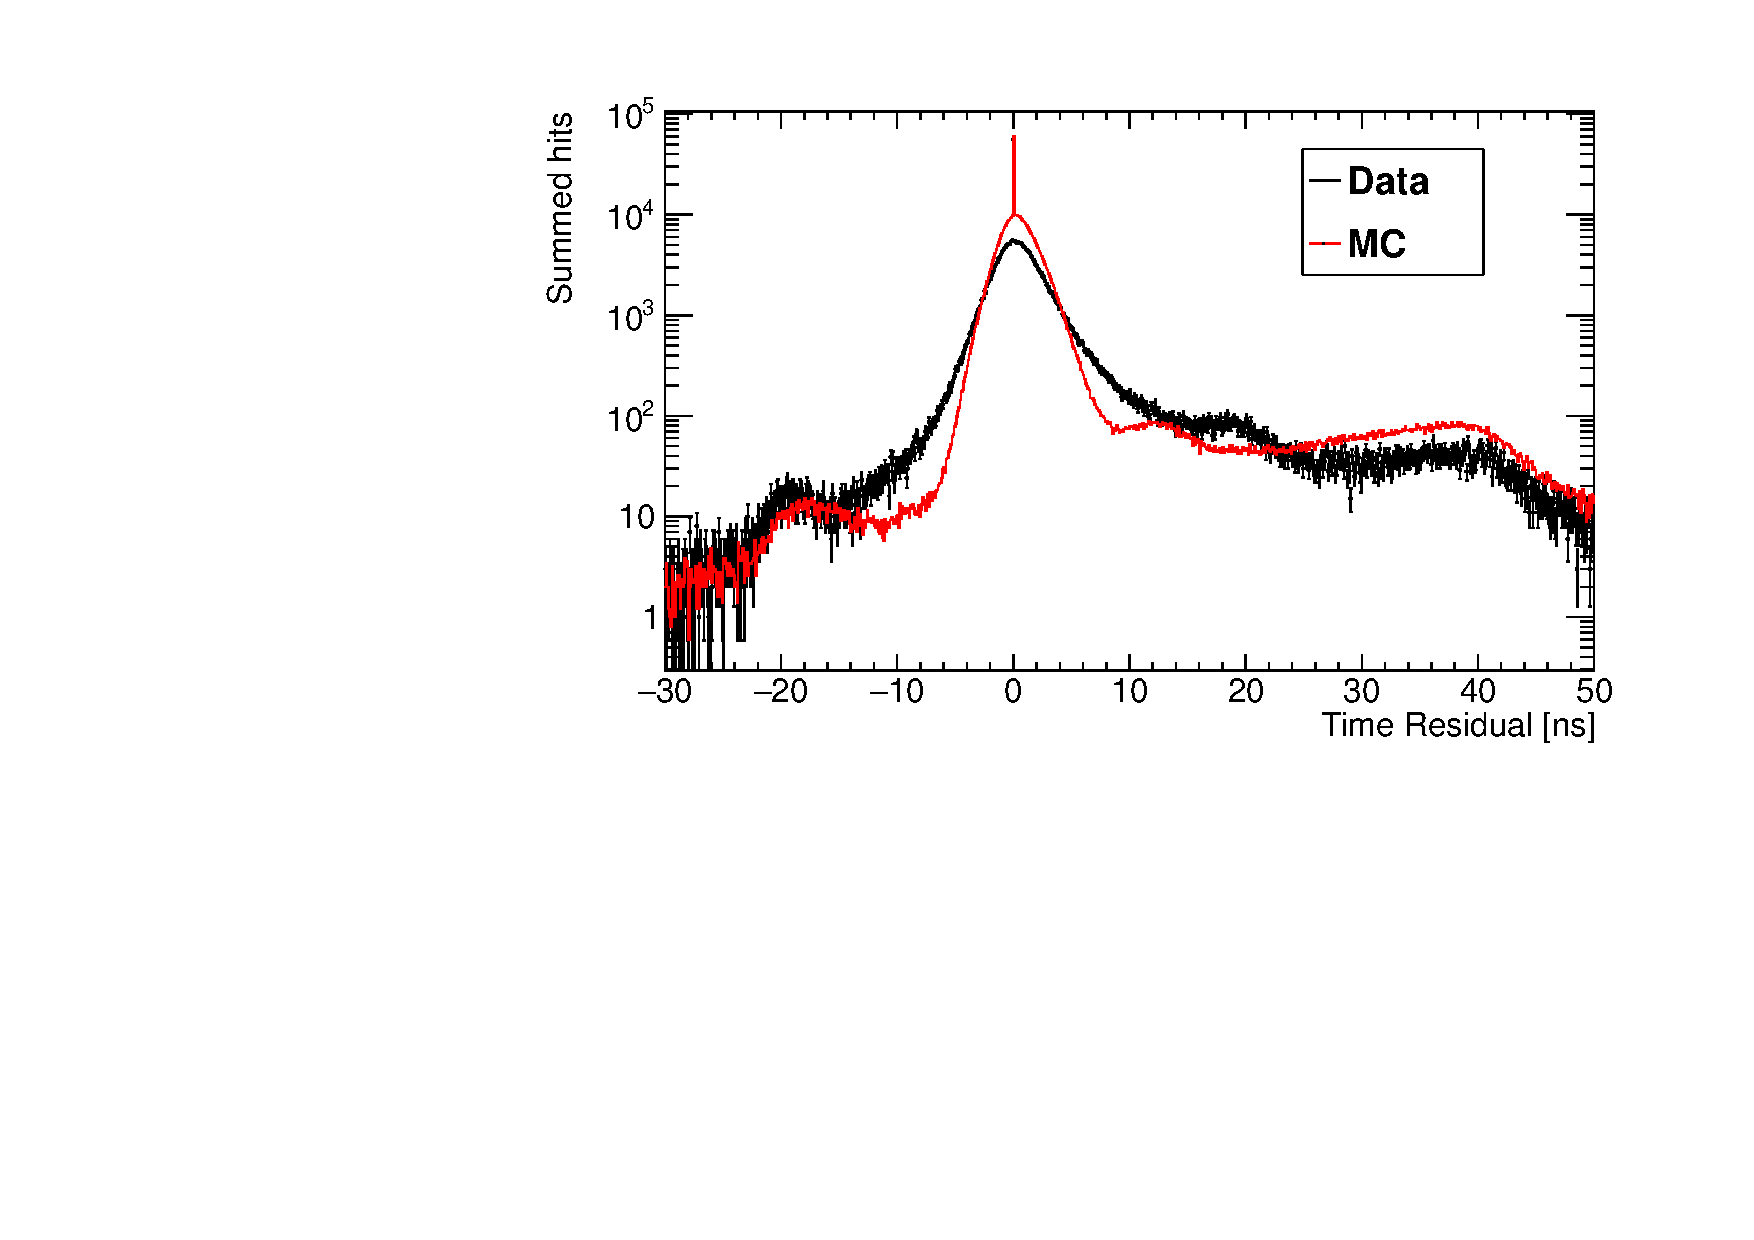
\includegraphics[width=\textwidth]{4_SMELLIESimulation/images/data_vs_mc_FS007_PQ495_nom_scatt_beamspot_tres_plot.pdf}
    \caption[Time residual distribution in the beamspot region for data taken in July 2022 with PQ495 through fibre FS007, as compared to a matching simulation]
    {Time residual distribution in the beamspot region for data taken in July 2022 with PQ495 through fibre FS007, as compared to a matching simulation. The width of the data's prompt peak is much broader than expected, and there is a notable bump at \SI{19}{\ns} not present in the MC.}
    \label{fig:smellie_pq495_prompt_timing_data_vs_mc}
\end{figure}

The two major discrepancies between data and MC seen for this laser is the much broader prompt peak seen in data than expected, and the bump at $\sim\SI{19}{\ns}$. Neither of these effects are seen in the other PQ lasers. Because these hits come almost exclusively from direct light, the most likely explanation for this difference is a change in the emission time distribution of the PQ495 laser, relative to the timing distributions used in \texttt{RAT} which were provided by the laser's manufacturer. One method for resolving this problem could be to measure the laser's emission timing distribution with an oscilloscope, in the same manner used by J. Lidgard to determine the timing distribution for the SuperK laser~\cite{lidgardSupercontinuumAdditionSMELLIE2018}.

    % \begin{itemize}
    %     \item For certain lasers, a strong mismatch in the observed hit time residuals for prompt light.
    %     \item A mysterious +18 ns bump seen for the PQ495 laser.
    %     \item A trigger jitter in the SuperK laser.
    % \end{itemize}
    % [3 pages]

\subsection{Backward Hemisphere Discrepancies}
A third class of systematic differences between data and simulation of SMELLIE events are those discrepancies observed in the distributions of hits near a given fibre emission point. Consider the region of 50 PMTs closest to a given fibre. This defines what shall be called the ``back-scatter'' region of PMTs, because these will be the PMTs which will see the greatest intensity of light that has Rayleigh scattered in the UPW outside the AV. For a given subrun, only the subset of these PMTs which were `good' in the sense described in Section~\ref{sec:combining_beam_profiles} were used. This PMT region will become useful to the analyses described in Chapter~\ref{chap:smellie_analysis}.

Fig.~\ref{fig:smellie_tres_back_data_vs_mc_water} shows the time residual distributions for data taken in water phase run \num{114018} in the back-scatter PMT region, using the SuperK laser in the wavelength range \SIrange{490}{500}{\nm}. The method of emission time calculation used here is that of $t_{\mathrm{med}}$. Because it is not possible for light to travel straight from the fibre emission point to a PMT in the back-scatter region, the light-paths used for calculating the time-of-flight in the time residuals here correspond to those which reflect off of the AV surface.  Also shown in these plots are matching simulations of these subruns. The distributions from simulation are displayed as stacked histograms, where each individual histogram corresponds to the subset of hits associated with photons that underwent specific types of path. The overall intensity of the simulation has been scaled so that the number of hits in the $[-30,-10]\,\si{\ns}$ time residual window is equal in data and MC, corresponding to a window in which only light that back-scattered in the outer water was observed.

\begin{figure}
    \centering
    \begin{subfigure}{0.98\textwidth}
        \centering
        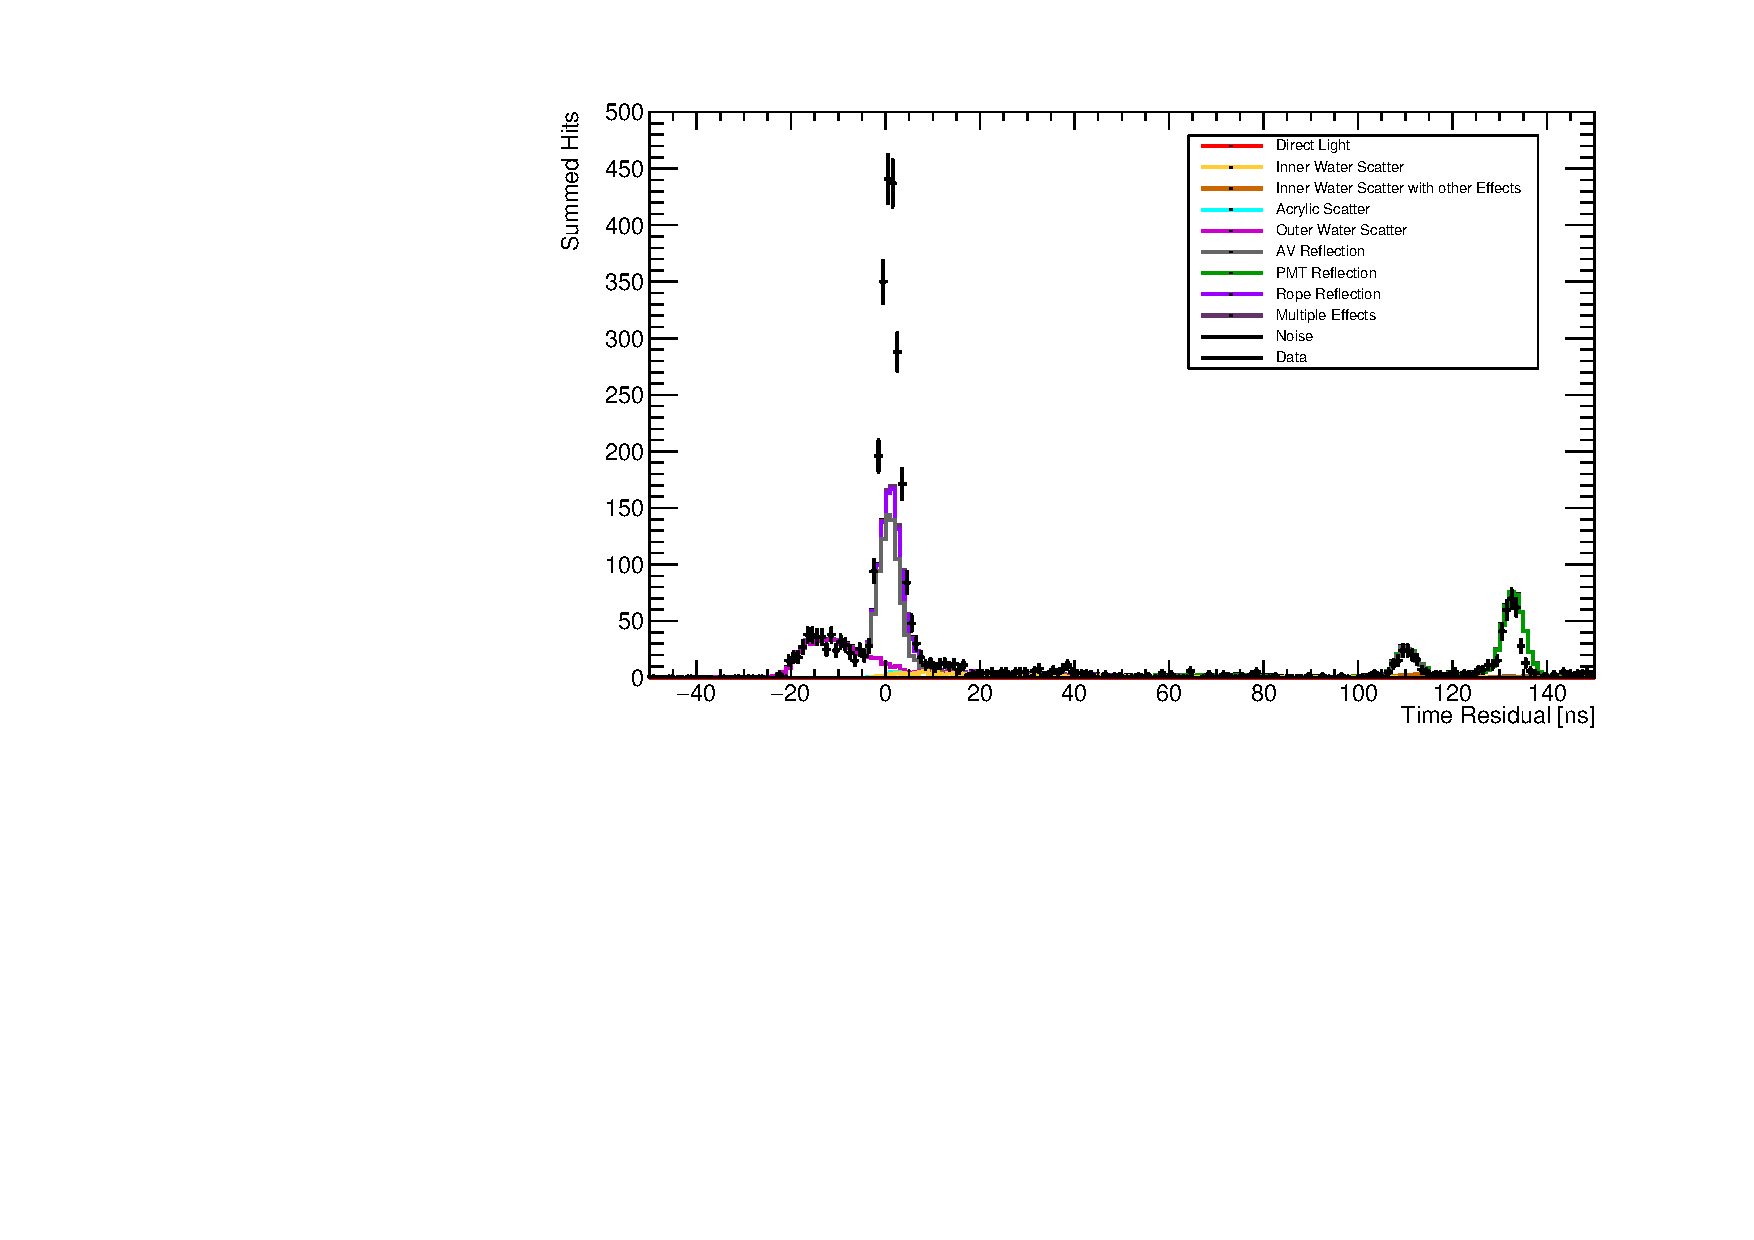
\includegraphics[width=\textwidth]{4_SMELLIESimulation/images/tres_plot_backscatter_water_FS007_SUPERK490_500_data_vs_mc_tracked.pdf}
        \caption{Fibre FS007}
        \label{fig:smellie_tres_back_data_vs_mc_fs007}
    \end{subfigure}
    \begin{subfigure}{0.98\textwidth}
        \centering
        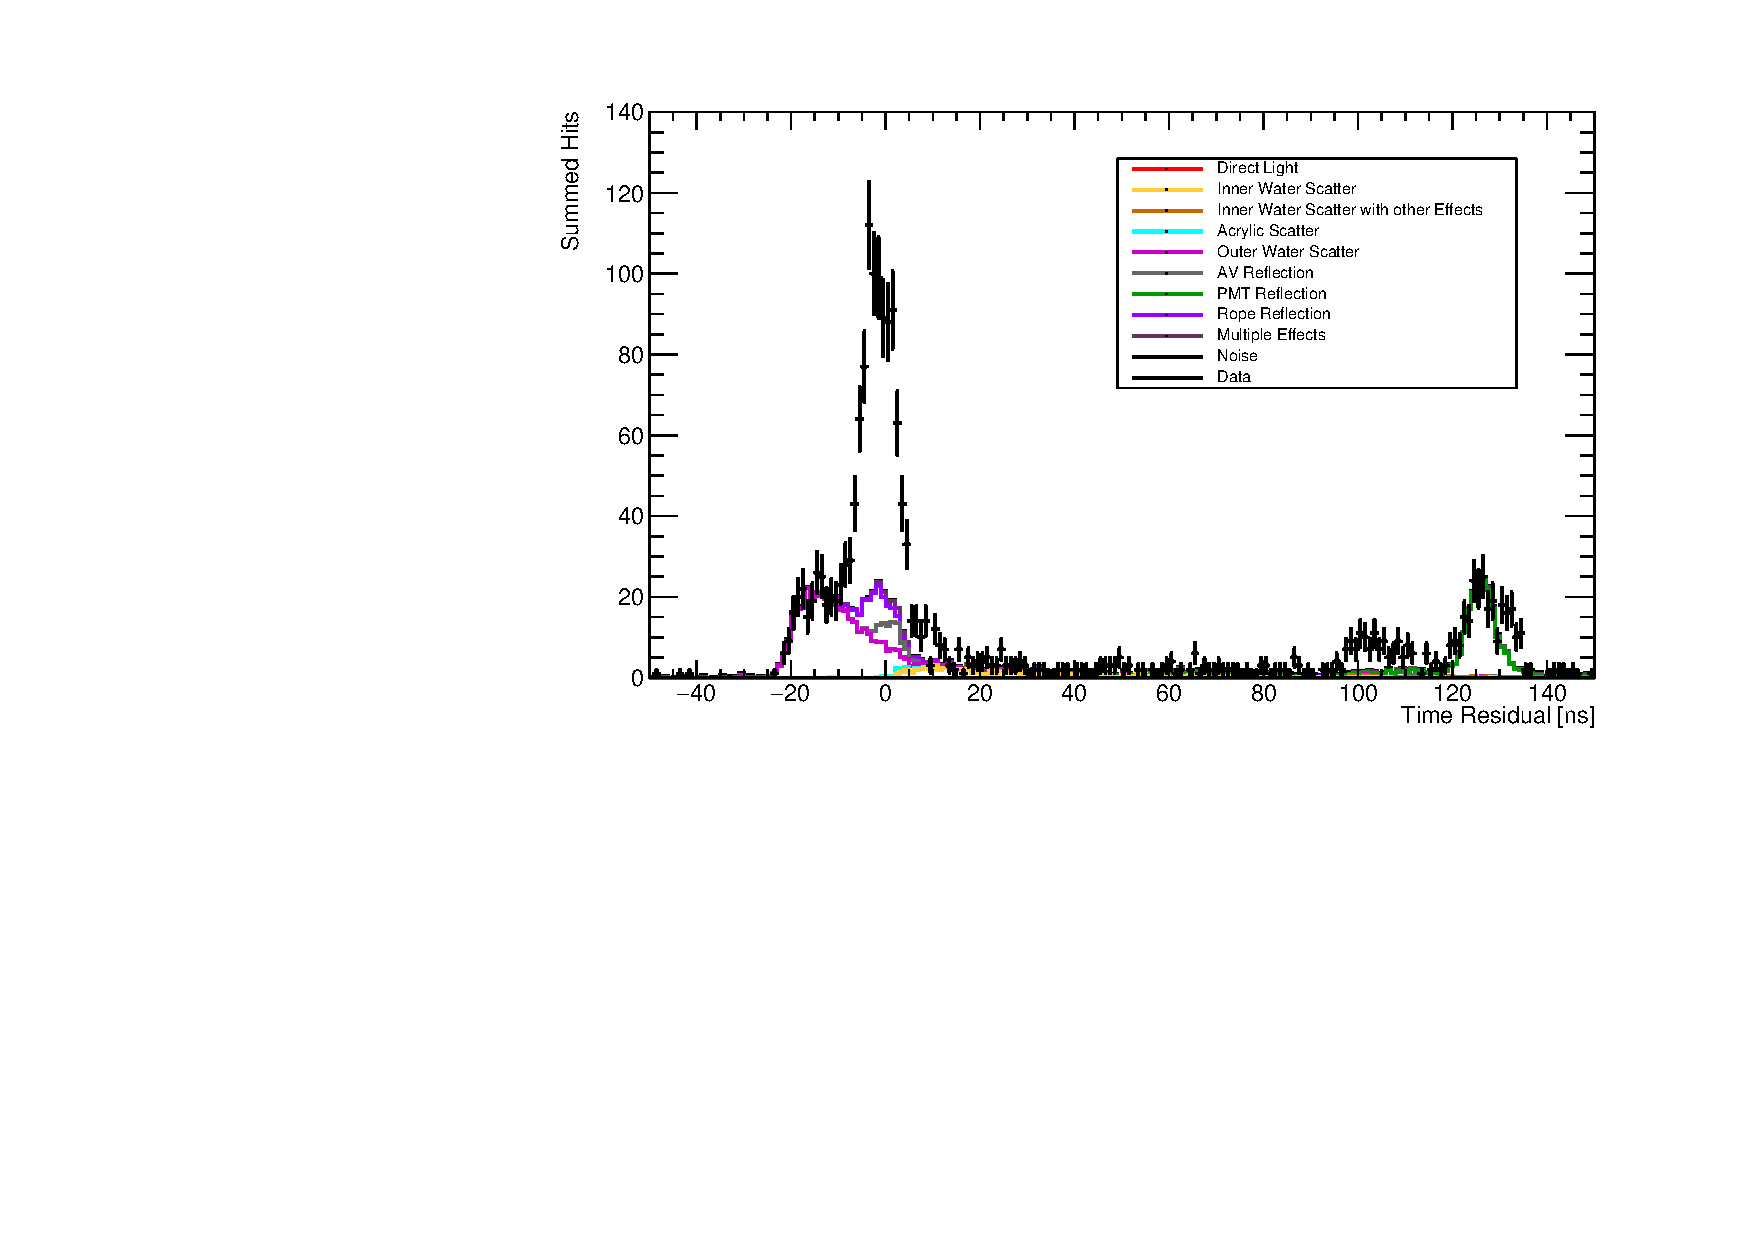
\includegraphics[width=\textwidth]{4_SMELLIESimulation/images/tres_plot_backscatter_water_FS155_SUPERK490_500_data_vs_mc_tracked.pdf}
        \caption{Fibre FS155}
        \label{fig:smellie_tres_back_data_vs_mc_fs155}
    \end{subfigure}
    \caption[Data--MC comparisons for water phase SMELLIE data in the back-scatter PMT region]
    {Plots showing comparisons between the time residual distributions in the `back-scatter' PMT region for water phase SMELLIE data taken in run \num{114018}, with the SuperK laser in the wavelength range \SIrange{490}{500}{\nm} for two different fibres, and matching MC.}
    \label{fig:smellie_tres_back_data_vs_mc_water}
\end{figure}

Looking at Fig.~\ref{fig:smellie_tres_back_data_vs_mc_fs007} in particular, corresponding to the \ang{0} fibre FS007, both data and simulation observe five distinct regions of interest. After the earliest peak from light which back-scattered in the outer water, there is a prominent peak near \SI{0}{\ns} arising from reflections off of the AV surface nearest to the fibre, as well as reflections from ropes. After this, in the \SIrange{10}{50}{\ns} range, there is a long tail of hits due to a number of effects, including back-scattering in the inner water. Much later, there are two further peaks: one at \SI{110}{\ns} due to reflections off of the far AV surface, and one at \SI{132}{\ns} due to reflections off of the PMTs and concentrators on the far side of the detector.

Although all the features described above are seen qualitatively in both data and MC, there are a couple of notable discrepancies. The first to note are the differences in shape seen in the PMT reflection peaks of both fibres shown. The FS007 data has a tighter peak than expected from simulation, whilst the FS155 data sees the opposite. These differences are likely due to the current limitations of the PMT reflection model used in \texttt{RAT}. Fig.~\ref{fig:smellie_laserball_late_light_data_vs_mc} shows the best-fit of Laserball data to simulations with varying PMT reflection models, taken from~\cite{andersonOpticalCalibrationSNO2021}. The last peak in this plot comes from PMT reflections, which shows a small disagreement between data and MC. It is presumably this residual systematic in the modelling of the PMT reflections that leads to the shape differences in the peaks seen in the SMELLIE data.

\begin{figure}
    \centering
    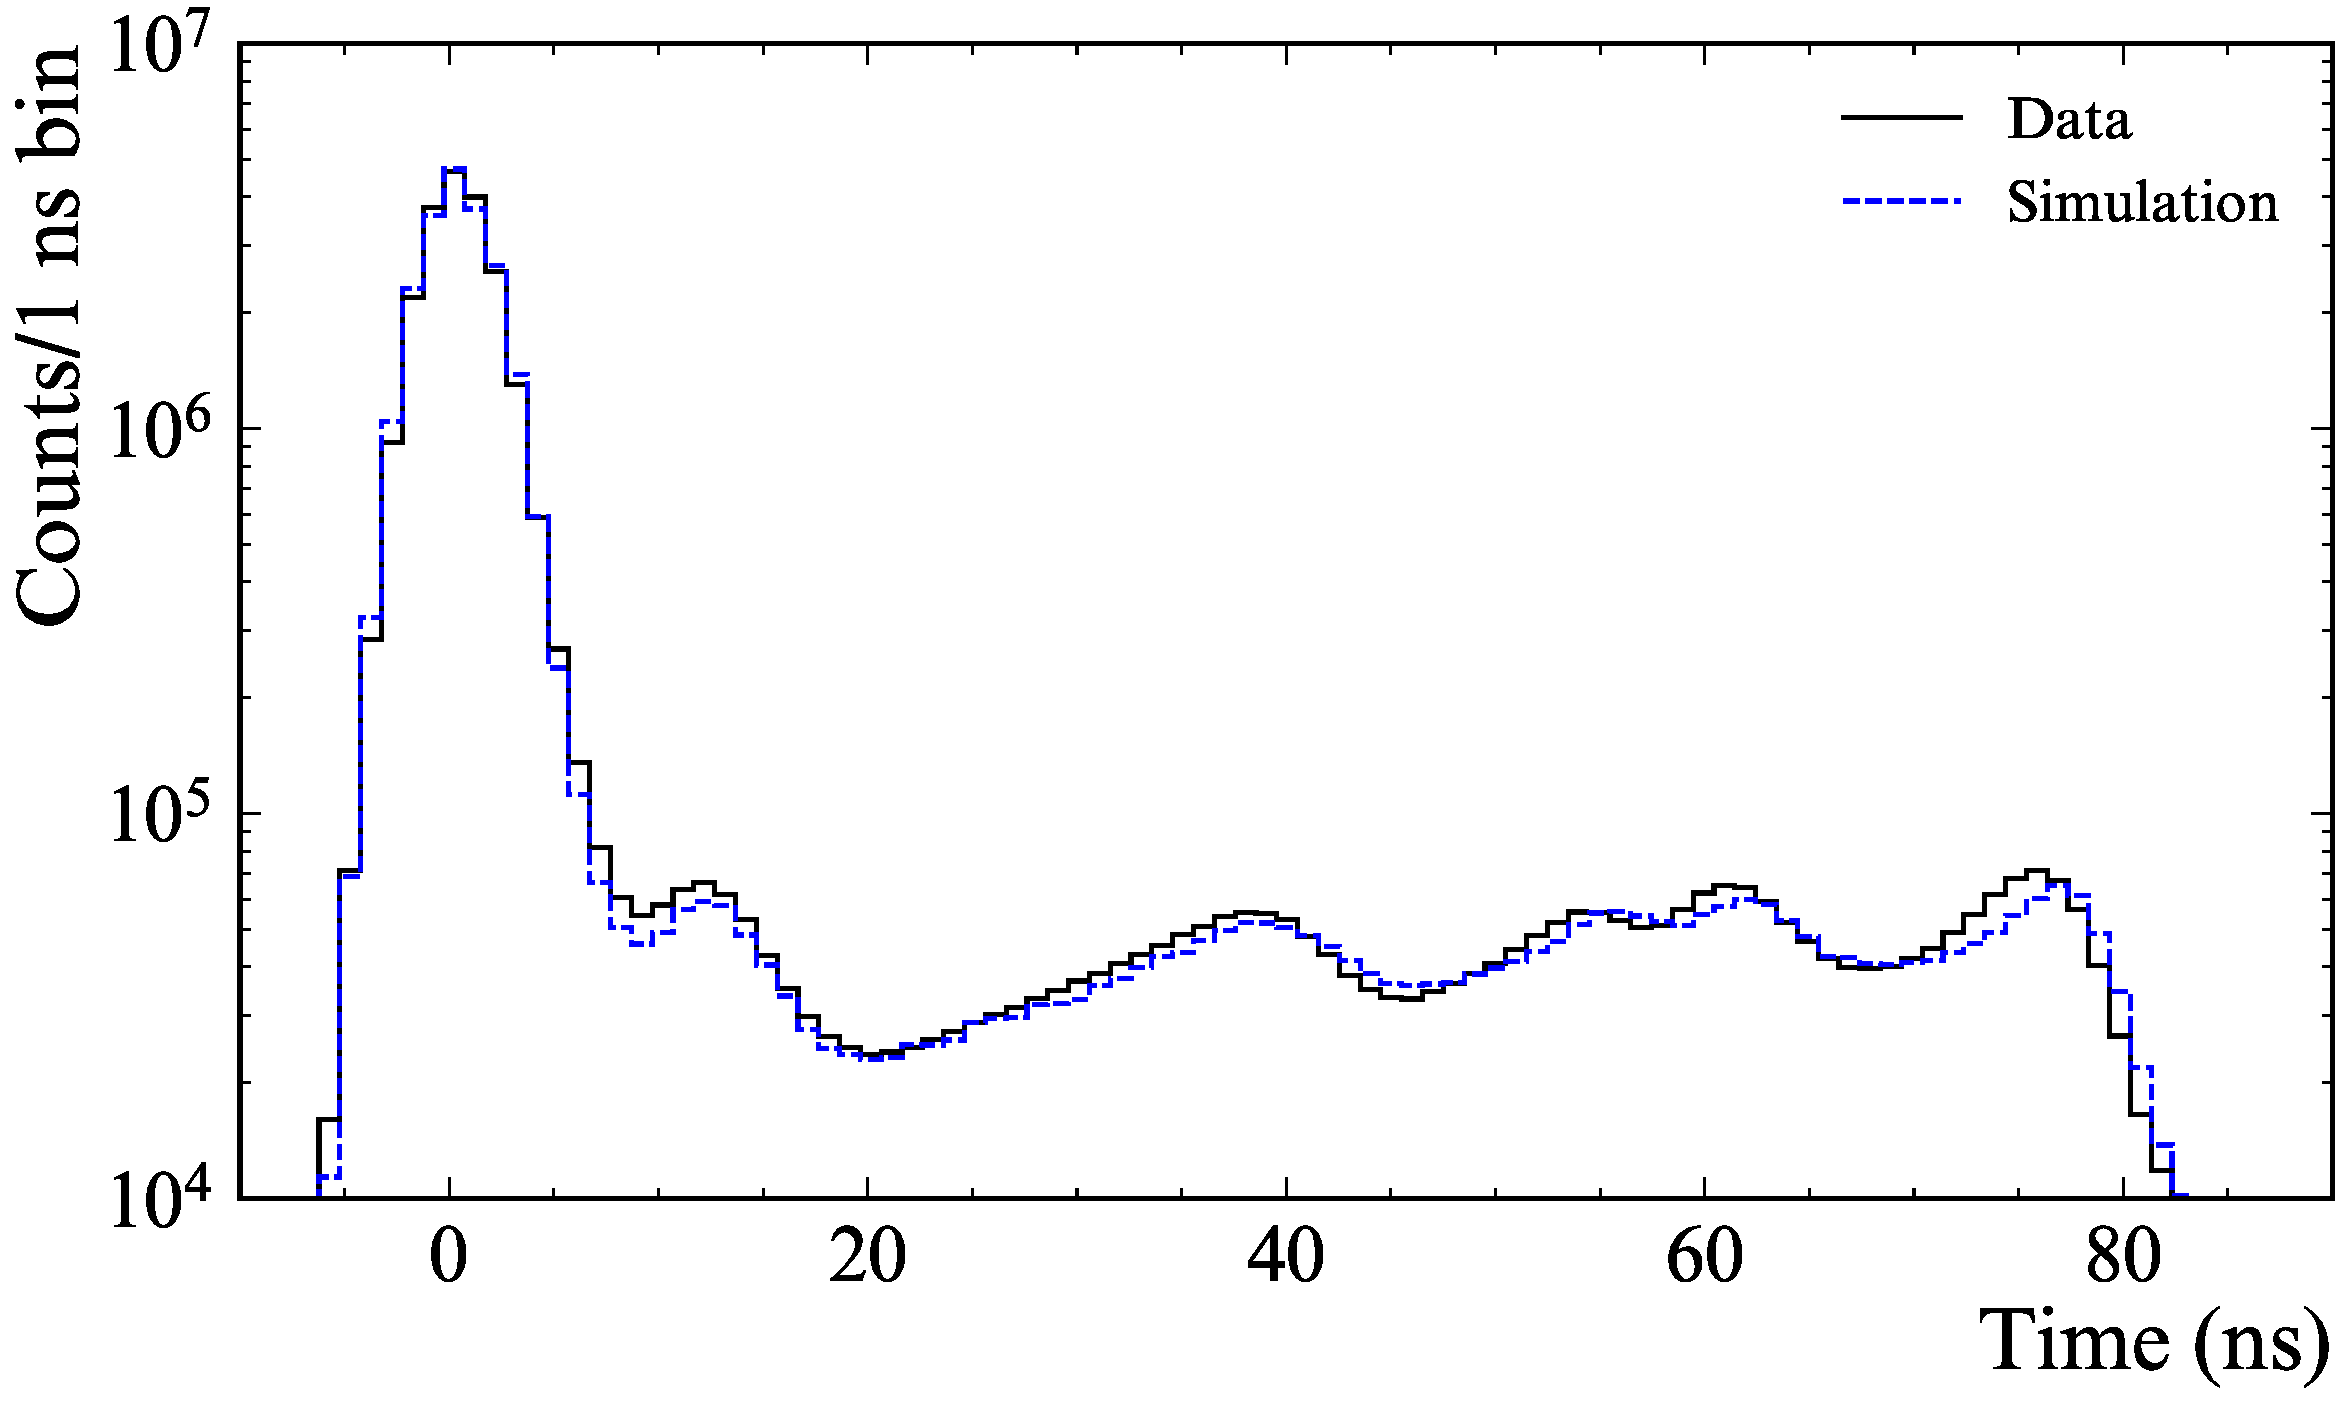
\includegraphics[width=\textwidth]{4_SMELLIESimulation/images/latelight.pdf}
    \caption[Comparison of Laserball data in the water phase to MC]
    {Comparison of Laserball data in the water phase to MC, with a wavelength of \SI{420}{\nm}. The latest peak comes from PMT reflections. From~\cite{andersonOpticalCalibrationSNO2021}.}
    \label{fig:smellie_laserball_late_light_data_vs_mc}
\end{figure}


The other prominent difference is the magnitude of the peak at \SI{0}{\ns}, with data appearing to have a peak over twice the size of simulation. This can clearly be seen for the results of both fibres in Fig.~\ref{fig:smellie_tres_back_data_vs_mc_water}. What could cause this discrepancy? One simple explanation is that the intensity calibration of the MC is wrong. Because the intensity of the simulation shown here has been forced to match that of the outer water back-scattered light, if the scattering length of this water is systematically off in simulation then so too would the intensity calibration. If this were the case, then the true Rayleigh scattering length of the outer water would have to be substantially longer than expected in order to explain the discrepancy in the peak at \SI{0}{\ns}. However, this would cause a substantial change in the magnitudes of the two later peaks. Given that these two late peaks have magnitudes which appear to agree with data under the current intensity calibration, a large systematic in the UPW scattering length does not seem like the primary cause of this systematic.

A second hypothesis for explaining the difference in peak heights at \SI{0}{\ns} is that there is far more light being reflected off of the AV surface than expected. As discussed in Section~\ref{sec:optical_processes}, standard specular reflection is entirely determined by the refractive indices of the two media, and the angle of incidence of the light. The refractive indices of the UPW and acrylic are well-known, and because FS007 is a \ang{0} fibre, the angles of incidence of light rays will be close to \ang{0} also. The fact that there appears to be good agreement between data and MC in the peak from reflections off of the far AV surface casts strong doubt on a substantial miscalculation of the specular reflection. An alternative theory is the existence of a diffusive reflection component on the AV surface, due to a surface roughness. This could possibly explain the existence of a peak seen in data in Fig.~\ref{fig:smellie_tres_back_data_vs_mc_fs155}, but not in the MC.

There are two further hypotheses which could possibly help to explain the \SI{0}{\ns} peak discrepancy. One is that the extra light in this peak comes from scattering in the acrylic, with the scattering length being much shorter than currently modelled. The current \texttt{RAT} model indicates that only a negligible fraction of light gets scattered in the acrylic, so there would need to be a dramatic change in the scattering length. The final hypothesis is that the rope reflections are currently being mismodelled. Currently, the model for rope reflections in \texttt{RAT} assumes 60\% reflectivity with the reflections being purely diffusive. However, this is based on preliminary estimates only, with no formal calibration to back this reflection model up. It could be the case that a different reflection model could help to alleviate the tension between data and model in the peak, although it is challenging to see how the all the difference could be attributed to purely this.

% {
% \color{blue}
%     \begin{itemize}
%         \item The observed distribution of hits vs time and angle in MC does not match data in a number of ways for PMTs near the fibre emission point.
%         \item Includes the outer-water scattering length, rope reflections, and investigations into whether certain modifications to the optics could plausibly fix things (so far, no).
%     \end{itemize}
%    [6 pages]

%    [32 PAGES TOTAL]
% }

\section{Summary and Suggestions for Further Work}
In this chapter, the simulation of SMELLIE events was updated in two ways. Firstly, a new algorithm for the generation of SMELLIE events was built, leading to a dramatic speed-up in simulation times of multiple orders of magnitude. This was achieved by converting a rejection sampling approach to sampling a fibre's beam profile into an `inverse-CDF'-style one, as well as pre-computing many calculations that were historically performed at run-time. The beam profiles were then updated by combining multiple datasets together, using a carefully-designed statistical model. By using substantially more data to build the beam profiles, a much greater dynamic range in the profiles was possible.

The updating of the beam profiles also uncovered a number of systematics still present in the simulations. By using interpolated forms of the new beam profiles, there is clear mismodelling in acrylic attenuation and the position of rope shadows. There is also a notable wavelength-dependence to the shape of the beam profiles. In addition, other data-MC discrepancies exist: the PQ495 laser has an observed emission time spectrum that does not match expectation, and there appears to be far more light coming from AV and/or rope reflections than expected, if one assumes that the modelling of the outer UPW scattering is correct. There are also differences in the shape of the time distributions of light reflected off of PMTs and their concentrators.

There are a number of things that can be done to further the work performed in this chapter. These come in two main classes: improvements to the SMELLIE generator, and improvements to the optical model of the detector in \texttt{RAT} more generally. For the former, the emission time distribution for the PQ495 laser should be measured external to the detector's DAQ, possibly using an oscilloscope. Alternatively, the PQ495 emission time distribution could be recovered by deconvolving the observed time distribution with the known PMT transit time distribution.

For the beam profiles, even more water phase data could be used if one were to include the `high' intensity data that was taken back in 2018, but never used. This would require some thought about how to appropriately handle PMTs which were fully-saturated: the npe would then have to be estimated by looking at the charge information. If one can work that out, then the benefit would be far greater statistics. In doing so, this would alleviate the reliance on combining beam profiles at multiple different wavelengths. Instead, separate beam profiles could be developed for different wavelengths, with the beam profile for a given simulated wavelength being the interpolation/extrapolation of these different beam profiles. It would also be beneficial to have a physical understanding of why this wavelength-dependence occurs.

However, the quality of the beam profile is fundamentally limited by the accuracy of the associated isotropic MC. This is linked to the second class of possible improvements: those of the optical model of the detector itself. In multiple beam profiles there are clear indications of rope shadows being incorrectly modelled. This could either come from the ropes being simulated in the wrong place, or the fibre emission points being incorrect, or a combination of both. By using the information from these beam profiles, it might be possible to determine where the ropes and fibres are. Also, the water phase SMELLIE data could be used to try and calibrate the optical models of the rope and PMT reflections.

There are indications of problems with the modelling of the acrylic optics from both the interpolated beam profile plots, and the time residual distributions of the back-scattered light region of PMTs. These could be related to the long-standing problem of attempting to model physics events near the AV --- for example, Iwan Morton-Blake saw in the partial fill phase that the \texttt{nhits} distribution of \ce{^{214}Bi-Po} radioactive background events had up to a 20\% difference in median value between data and MC near the AV~\cite{morton-blakeFirstMeasurementReactor2021}. More information about this background can be found in Section~\ref{sec:background_processes}. A similar effect was seen in the main scintillator phase by T. Zummo~\cite{zummoResidualEnergyCorrection2023}. Investigating different models of the acrylic optics to fix these systematic problems is worthwhile not just for SMELLIE, but for the experiment more broadly. It would be important to make sure that any optical model changes would maintain consistency with the data taken by the Laserball.